\documentclass[10pt,a4paper]{article} 
%\documentclass[10pt,a4paper,twocolumn]{article} 

% preamble
\input{00_preamble.tex}

% Coverpage setup
\title{ Systems Security (F25.520212U009.A) \\
        Project 02 \\
        Group 5 \\
        Aarhus University%
}

\author{Miklos Daniel Vadasz}


\begin{document}

\maketitle\thispagestyle{empty}
\makeatletter

\newpage
\tableofcontents\thispagestyle{empty}
\lstlistoflistings
%\listofalgorithms
\newpage

% Abastract for Mini TLS-based VPN tunelling
\thispagestyle{empty}
\begin{abstract}

\begin{center}
    \textbf{Mini TLS-based VPN tunneling}
\end{center}

%%% 
A Virtual Private Network (VPN)\cite{network.vpn} is a private network built on top of a public network, usually the Internet.
Computers inside a VPN can communicate securely, just like if they were on a real private network that is
physically isolated from outside, even though their traffic may go through a public network.

Virtual Private Networks enables employees to securely access a company’s intranet while traveling, it also allows companies to expand their private networks to places across the country and around the world.

The objective of this task was to implement a small VPN tunneling program that will allow hosts to communicate over an encrypted connection by modifying the provided code snippets by SEED Labs (please refer to: \cite{seedlab2024}).

In the final step the task was to replace the UDP socket with a TLS/SSL connection. To be able to generate the client/server cerfitications I used the openssl library, with respect to the deployed certificate structure.  

For \textit{mTLS}\cite{network.mtls} I choosed to use common self-signed certificate which were available on endpoints \lstinline{vpn-client-10.9.0.12} and \textit{vpn-server-10.9.0.11} respectively.

To be able to collect/analyze evidence regarding the network packets between endpoints I used common networking tools such as tcpdump\cite{bin.tcpdump}, tshark\cite{bin.tshark} and wireshark\cite{wiresharkorg} on the pre-configured interfaces (\textit{tun0}, \textit{eth0}, \textit{eth1}) after setting up the \textit{TLS}\cite{tls13security} tunnel. 
\end{abstract}

\newpage

\setcounter{page}{1}

% Reproducing the Seed LAB Exercises
\section{Lab Environment and Interface Setup}

\subsection{Network Setup}
\label{ssec:seed-network-setup}
%%%%%

I will create a VPN tunnel between a computer (client) and a gateway, allowing the computer to securely access a private network via the gateway. To be able to do that I will need at least three "machines": VPN client, VPN server (the router/gateway), and a host in the private network. 

%%%
The network topology according to \textit{\ref{fig:labtest}} can be seen on figure \textit{\ref{fig:networktopology}}.


\begin{figure}[h]
    \centering
    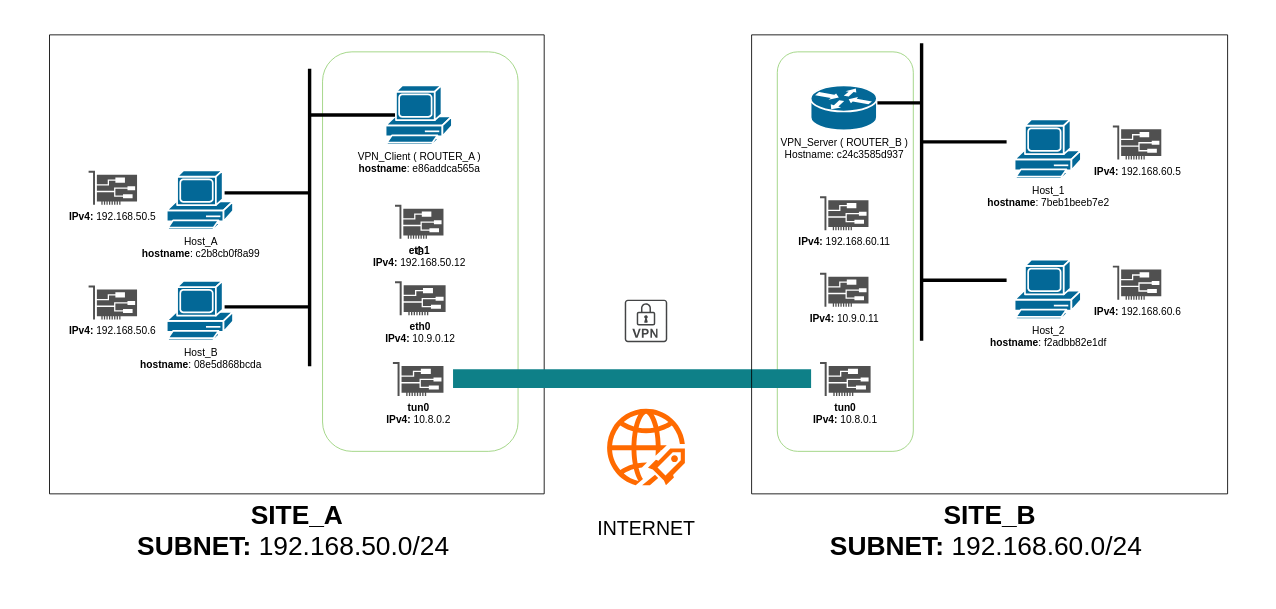
\includegraphics[width=0.65\linewidth]{Picture/02_Lab-exercises/netlab-topology.drawio.png}
    \caption{A possible network topology  based on the container environments}
    \label{fig:networktopology}
\end{figure}


(\textit{Please note:} Since I ran into compatibility issues with \textit{Scapy version 2.6.1} (please refer to \ref{apx:scapy-issue}) I rewrote the last , tls tunneling part, but since the original task was built upon \textit{SEED Lab}'s lab excercise I wanted to keep this whole part as well up until \textit{Section \ref{ssec:tunnl.send}}.  )

In practice, the VPN client and VPN server are connected via the Internet. For the sake of simplicity, I directly connect these two machines to the same LAN in this lab, i.e., this LAN simulates the Internet.
The "third machine", \textit{host-192.168.60.5} , is a computer inside the private network. The basic exercise showcases that the users on \textit{Site A} wants to communicate with users on \textit{Site B} via a VPN tunnel trough the interface \lstinline{tun0}.


The following image (\textit{\ref{fig:labtest}}) showcases a running environment with the following defined networks using CIDR notation : \textit{192.168.50.0/24}, \textit{192.168.60.0/24}, \textit{10.9.0.0/24}

\begin{figure}[h]
    \centering
    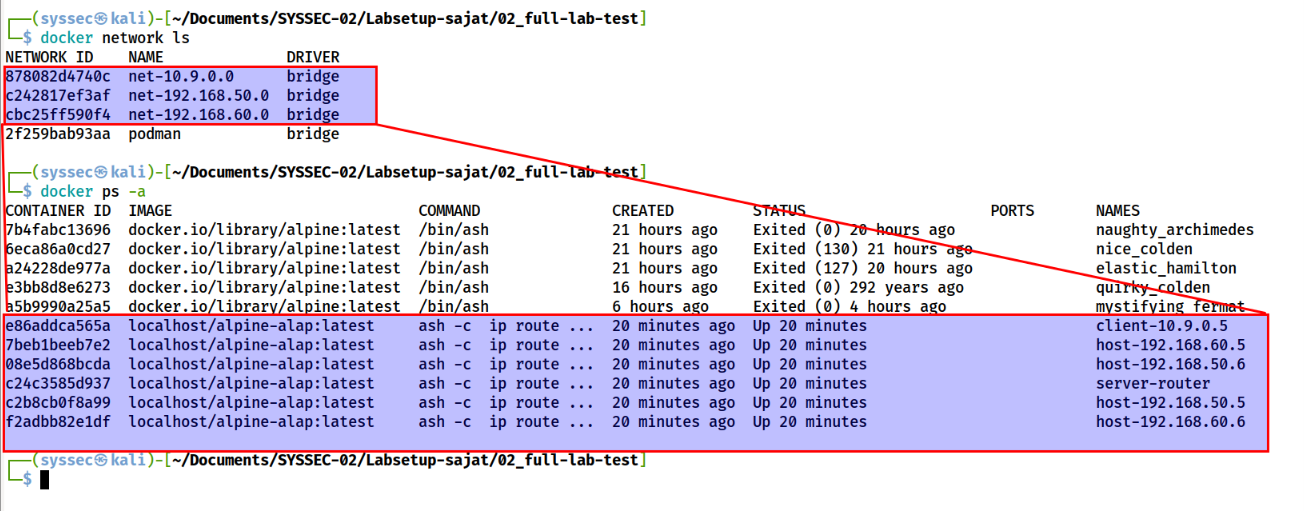
\includegraphics[width=0.65\linewidth]{Picture/00_Lab-Environment_Setup/00_running-lab.png}
    \caption{A running lab environment for Seed Lab's \textit{Exercise 2} built from \textit{LAB-VPN.yml}}
    \label{fig:labtest}
\end{figure}

To be able to assign one host to a network segment I made the following code snippet (to see the full solution, please refer the Appendix \ref{apx:lab__building-the-complete-lab-environment}) regarding the \textit{Dockerfiles}\cite{docker.dockerfiles}:

\begin{lstlisting}[caption=Definition of network subnet \lstinline{192.168.50.0/24}]
...
     networks:
            net-192.168.50.0:
                ipv4_address: 192.168.50.5
...
\end{lstlisting}

In order to be able to share files within the VM (Kali) and container images I have created a shared folder between the VM and the container using the Docker \lstinline{volumes}. This way the shared folder will be mounted as \lstinline{/volumes/} within the containers \lstinline{vpn-client-10.9.0.12} and \lstinline{vpn-server-10.9.0.11}. 

\begin{lstlisting}[language=bash, caption=Mount shared folders with host within the  container]
volumes:
    - ./volumes:/volumes
\end{lstlisting}

Futheron I'll use the folder \lstinline{./volumes} as an output folder for connectivity rest results, shere scripts with containers, etc.  This way the necessary codes in the  folder (on the VM) can be used inside the containers while being editable on the host (\textit{Kali}) machine as well, showed on \textit{figure \ref{fig:shared}}.

\begin{figure}[h]
    \centering
    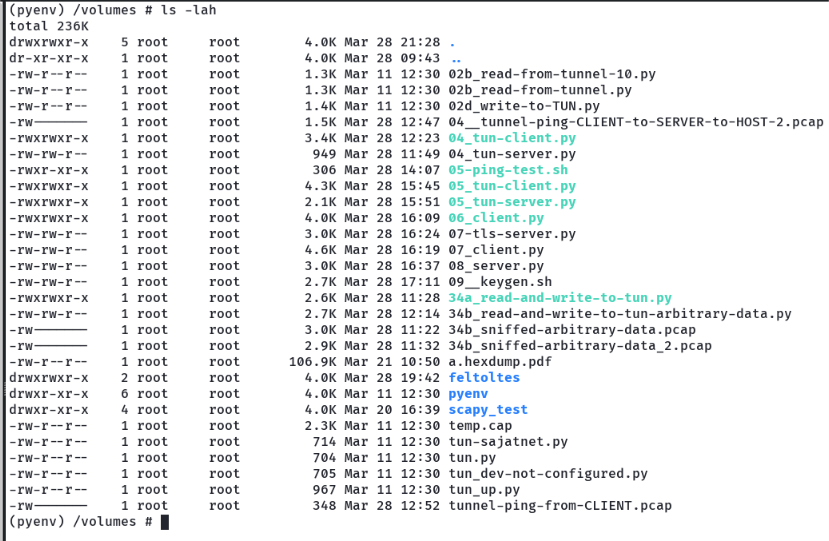
\includegraphics[width=0.3\linewidth]{Picture/02_Lab-exercises/volumes-directory.pdf.png}
    \caption{Shared folder between the Host System and Container Images}
    \label{fig:shared}
\end{figure}

To be able to sniff packets on a given interface (e.g.: \textit{eth0}) I used several networking tools, including \textit{tcpdump}\cite{bin.tcpdump}, \textit{tshark}, and the builtin method \lstinline{sniff()} from the library \lstinline{scapy}\cite{scapy}. 

I  have already installed \textit{tcpdump} on the container image (\lstinline{alpine:latest}) during build time (please refer to: \textit{Appendix \ref{apx:lab__install-packages-container}}) so to sniff the packets going through a particular interface, I just need to find out the interface name e.g. with \textit{ip addr} (see \textit{figure \ref{fig:ifname-before-tun}}  ) and choose the parametrization for \lstinline{tcpdump} as follows:

\begin{lstlisting}[language=bash, caption=Sniffing traffic on eth0 interface with tcpdump]
# Sniffing ICMP packets on in
tcpdump -i eth0 -n    
\end{lstlisting}

It should be noted that inside containers, due to the isolation created by Podman, when I run \textit{tcpdump} inside a container, I will be able only sniff the packets going in and out of that particular container. 

\begin{figure}[h]
    \centering
    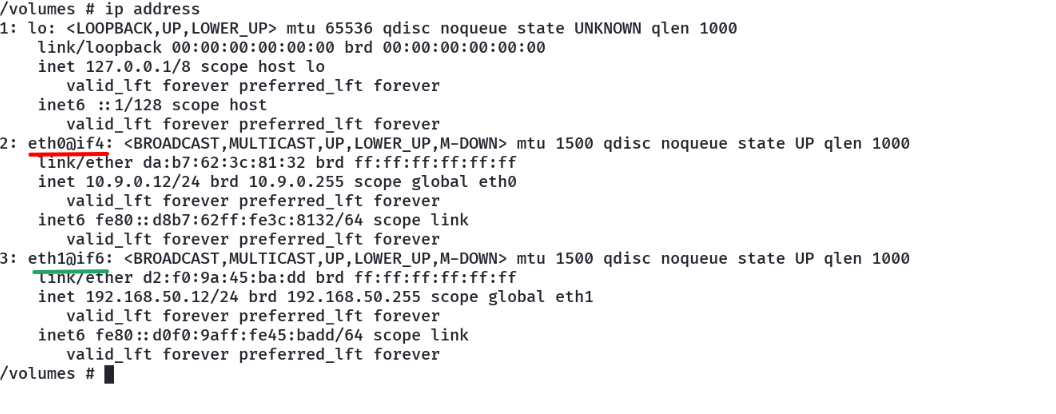
\includegraphics[width=0.65\linewidth]{Picture/02_Lab-exercises/00_if-names_before-tunnel.pdf.png}
    \caption{Listing the available interfaces with the command \textit{ip addr} on a given container host.}
    \label{fig:ifname-before-tun}
\end{figure}

After activating the python environment on a given host ( \lstinline{source /volumes/pyenv/bin/activate}) I can use scapy to sniff packets on the chosen interface (e.g.: \textit{eth0}) and write it to \textit{pcap} file for further analysis. The following code snippet showcases this scenario based on \cite{seedsecuritylab}:

\begin{lstlisting}[language=python, caption=Sniffing IP traffic with Scapy on interface eth0]
    from scapy.all import *
....

# Sniff ten packets on interface" `eth0`
# Display the raw bytes in the form "SOURCE_IP" -> "DESTINATION_IP" 
pkts_test = sniff(iface="eth0",prn=lambda x:x.sprintf("{IP:%IP.src% -> %IP.dst%\n}{Raw:%Raw.load%\n}"), count = 10)

# Write out the sniffed packat to `10packets.cap` file
wrpcap("10packets.cap",pkts_test)
\end{lstlisting}

\subsection{Testing the Network Connectivity Between Containers}

For the connectivity test regarding capturing packets I used \textit{tcpdump} in conjunction with \textit{tshark}, showcased on \textit{Figure \ref{fig:host-subnet}} 

\begin{table}[h!]
\centering
\begin{tabular}{|l|l|l|l|l|l|}
\hline
\textbf{Container Name} & \textbf{Hostname} & \textbf{Networks} & \textbf{Gateway} & \textbf{IPv4} & \textbf{MAC} \\
\hline
client-10.9.0.5 & * & net-10.9.0.0 & 10.9.0.1 & 10.9.0.12 & * \\
client-10.9.0.5 & * & net-192.168.50.0 & 192.168.50.1 & 192.1680.50.12 & * \\
\hline
Server-router & * & net-10.9.0.0 & 10.9.0.1 & 10.9.0.11 & * \\
Server-router & * & net-192.168.60.0 & 192.168.60.1 & 192.168.60.11 & * \\
\hline
host-192.168.50.5 & * & net-192.168.50.0 & 192.168.50.1 & 192.168.50.5 & * \\
host-192.168.50.6 & * & net-192.168.50.0 & 192.168.50.1 & 192.168.50.6 & * \\
\hline
host-192.168.60.5 & * & net-192.168.60.0 & 192.168.60.1 & 192.168.60.5 & * \\
host-192.168.60.6 & * & net-192.168.60.0 & 192.168.60.1 & 192.168.60.6 & * \\
\hline
\end{tabular}
\caption{Network Configuration for Containers. I ommited the fields \textit{hostname} and \textit{MAC} since these values are generated randomly. }
\label{tab:topology}
\end{table}

In the following few figures I collected the results of the following test cases:
Containers are able to reach eachother on a given subnet (figure \ref{fig:host-subnet})

%%% %%%%%%%%%%%%%%%%%%%%%%%%%%%%%%%%%%%%%%%% rrrr
Please note: I wrote this part of the report according to Seed Lab's exercises and tasks, for the complete bi-directional test with \lstinline{TLS} tunnel please refer to \textit{Section }


\begin{figure}[h]
    \centering
    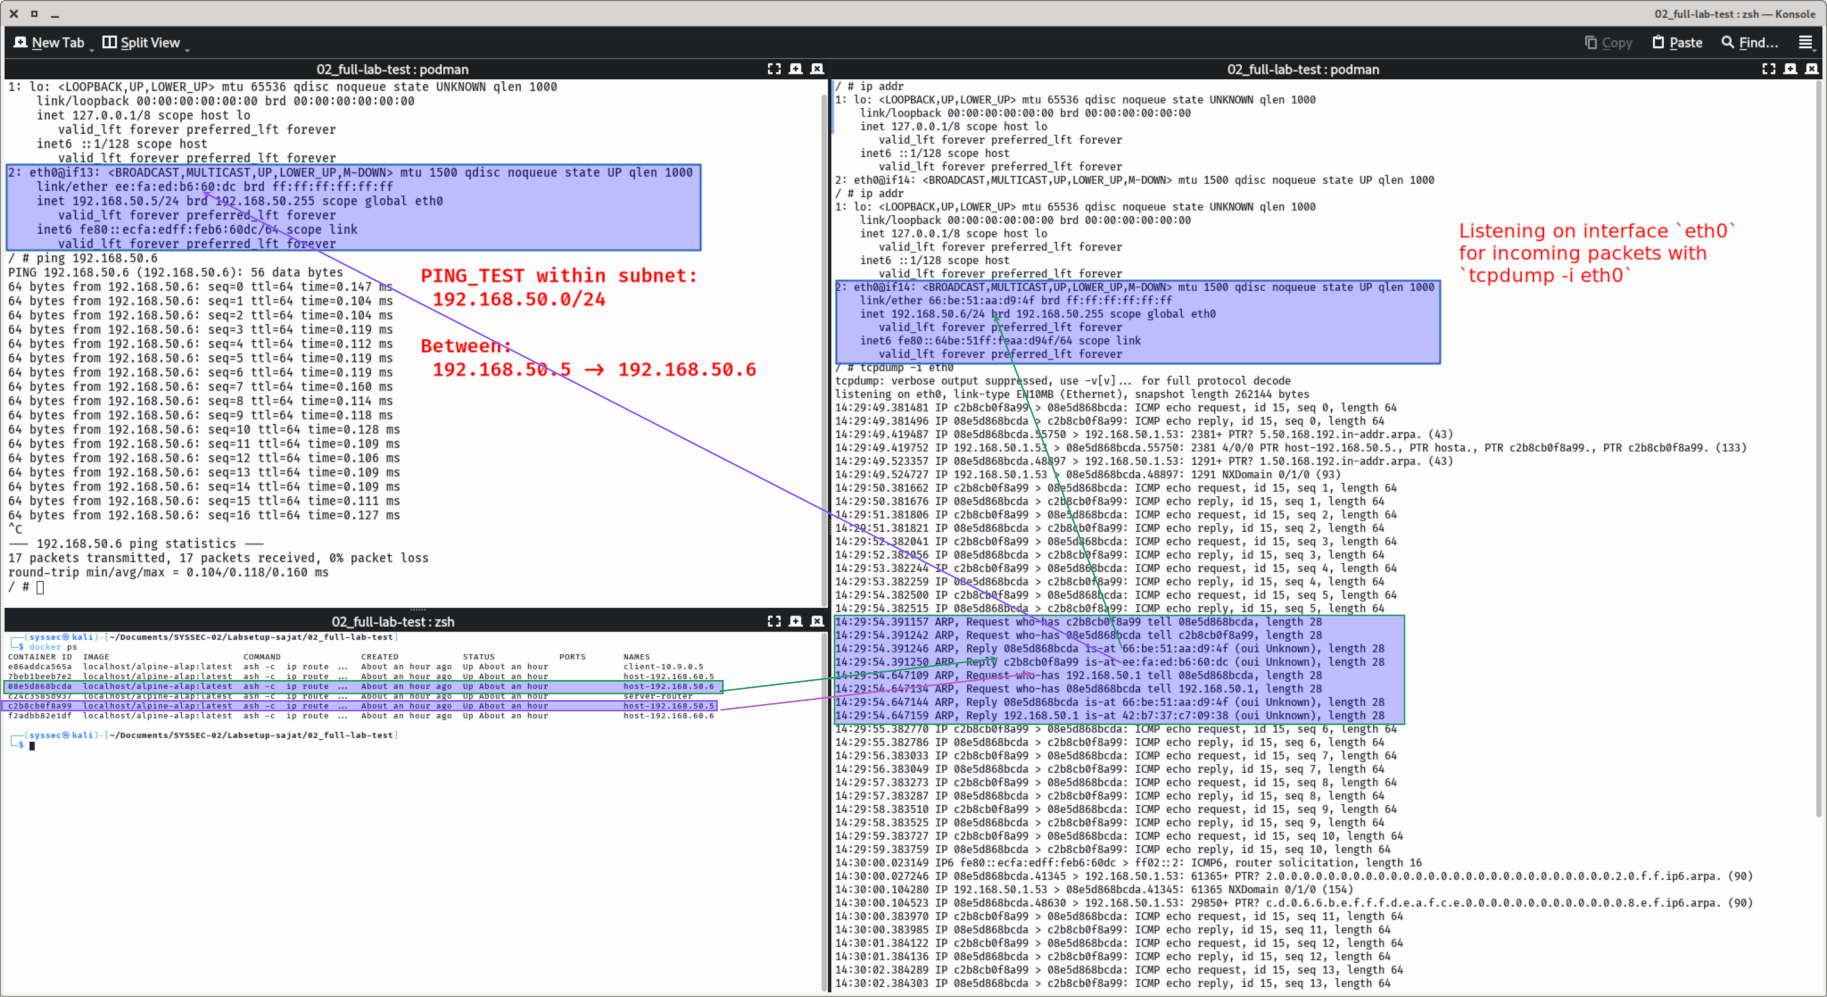
\includegraphics[width=0.65\linewidth]{Picture/02_Lab-exercises/020_connectivity-test/02_running-lab-test__network-PINGtest-ARP-requests.pdf.png}
    \caption{Hosts are able to reach eachother within the same subnet. }
    \label{fig:host-subnet}
\end{figure}

Figure \ref{fig:diffsubnet} shows that different hosts within a different subnet (namely \textit{Site A} and \textit{Site B}) are not able to reach each other, yet.

\begin{figure}[h]
    \centering
    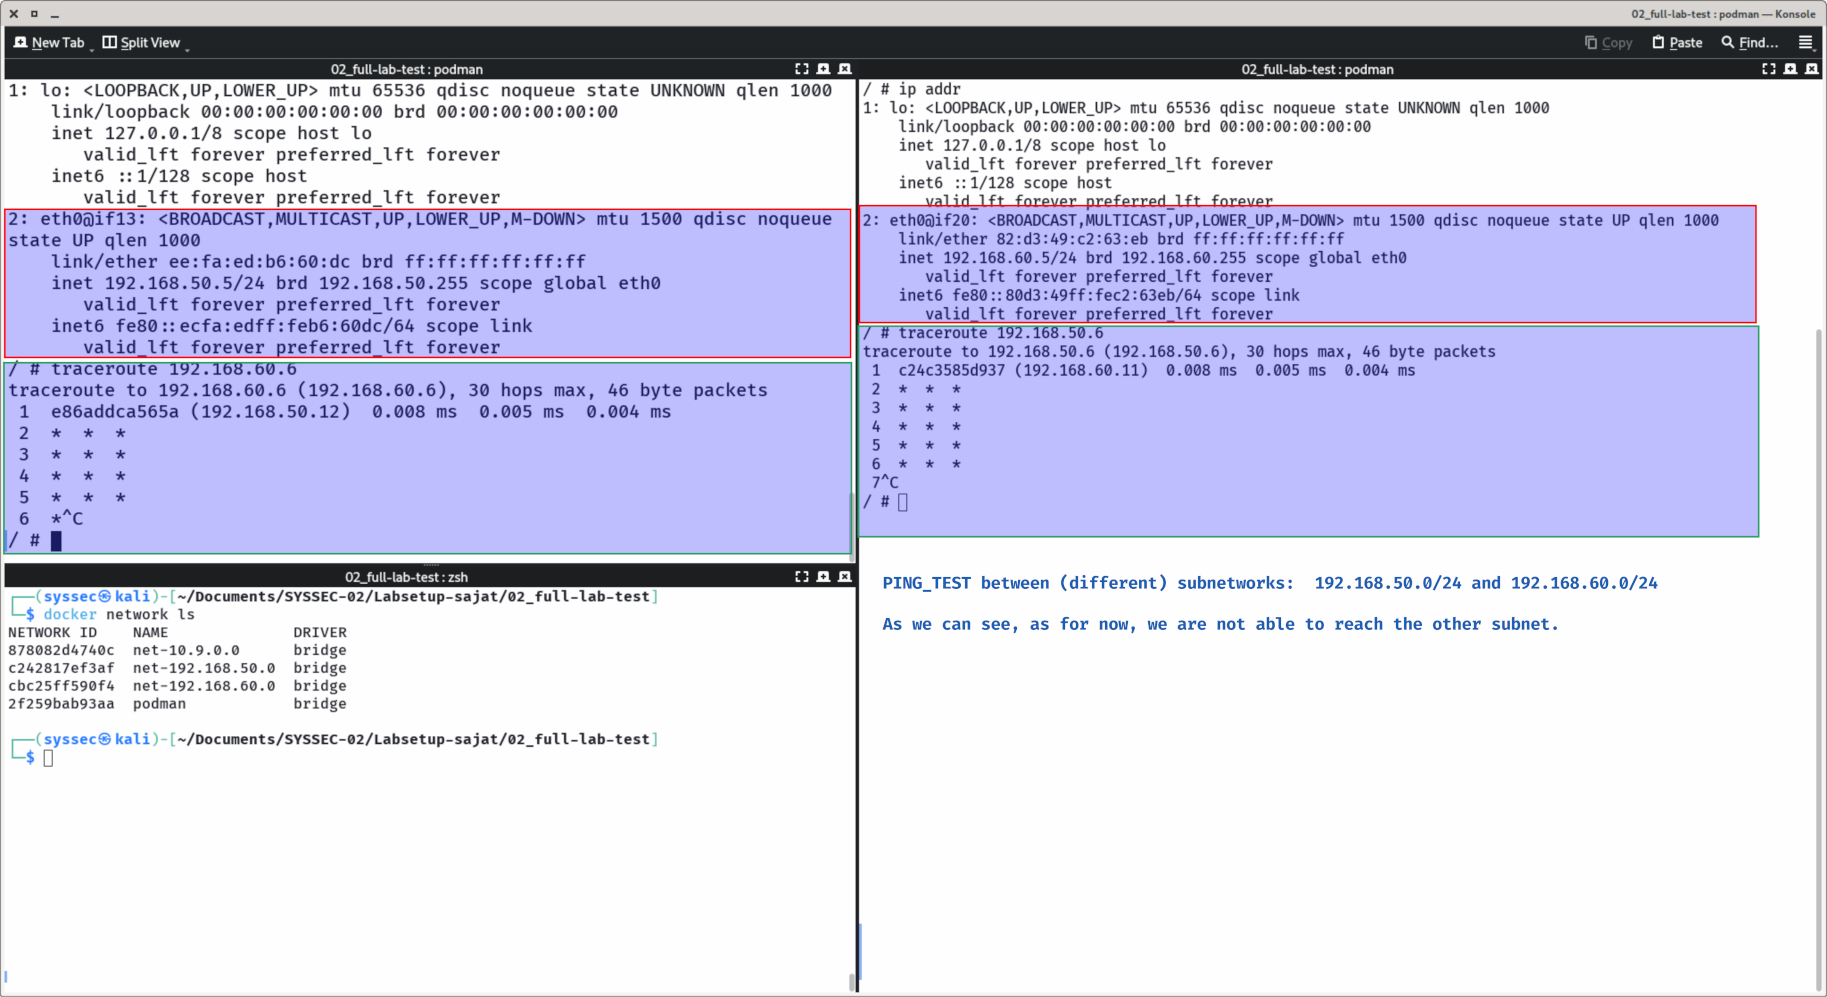
\includegraphics[width=0.65\linewidth]{Picture/02_Lab-exercises/020_connectivity-test/03_LAB-TEST__02-different-subnet-ping-test.pdf.png}
    \caption{Host within different subnets are not reachable}
    \label{fig:diffsubnet}
\end{figure}

Figure \ref{fig:vpn-server-reach} shows that Host 192.168.50.5 (which also assigned to \textit{10.9.0.11}) can communicate with VPN Server: 

\begin{figure}[h]
    \centering
    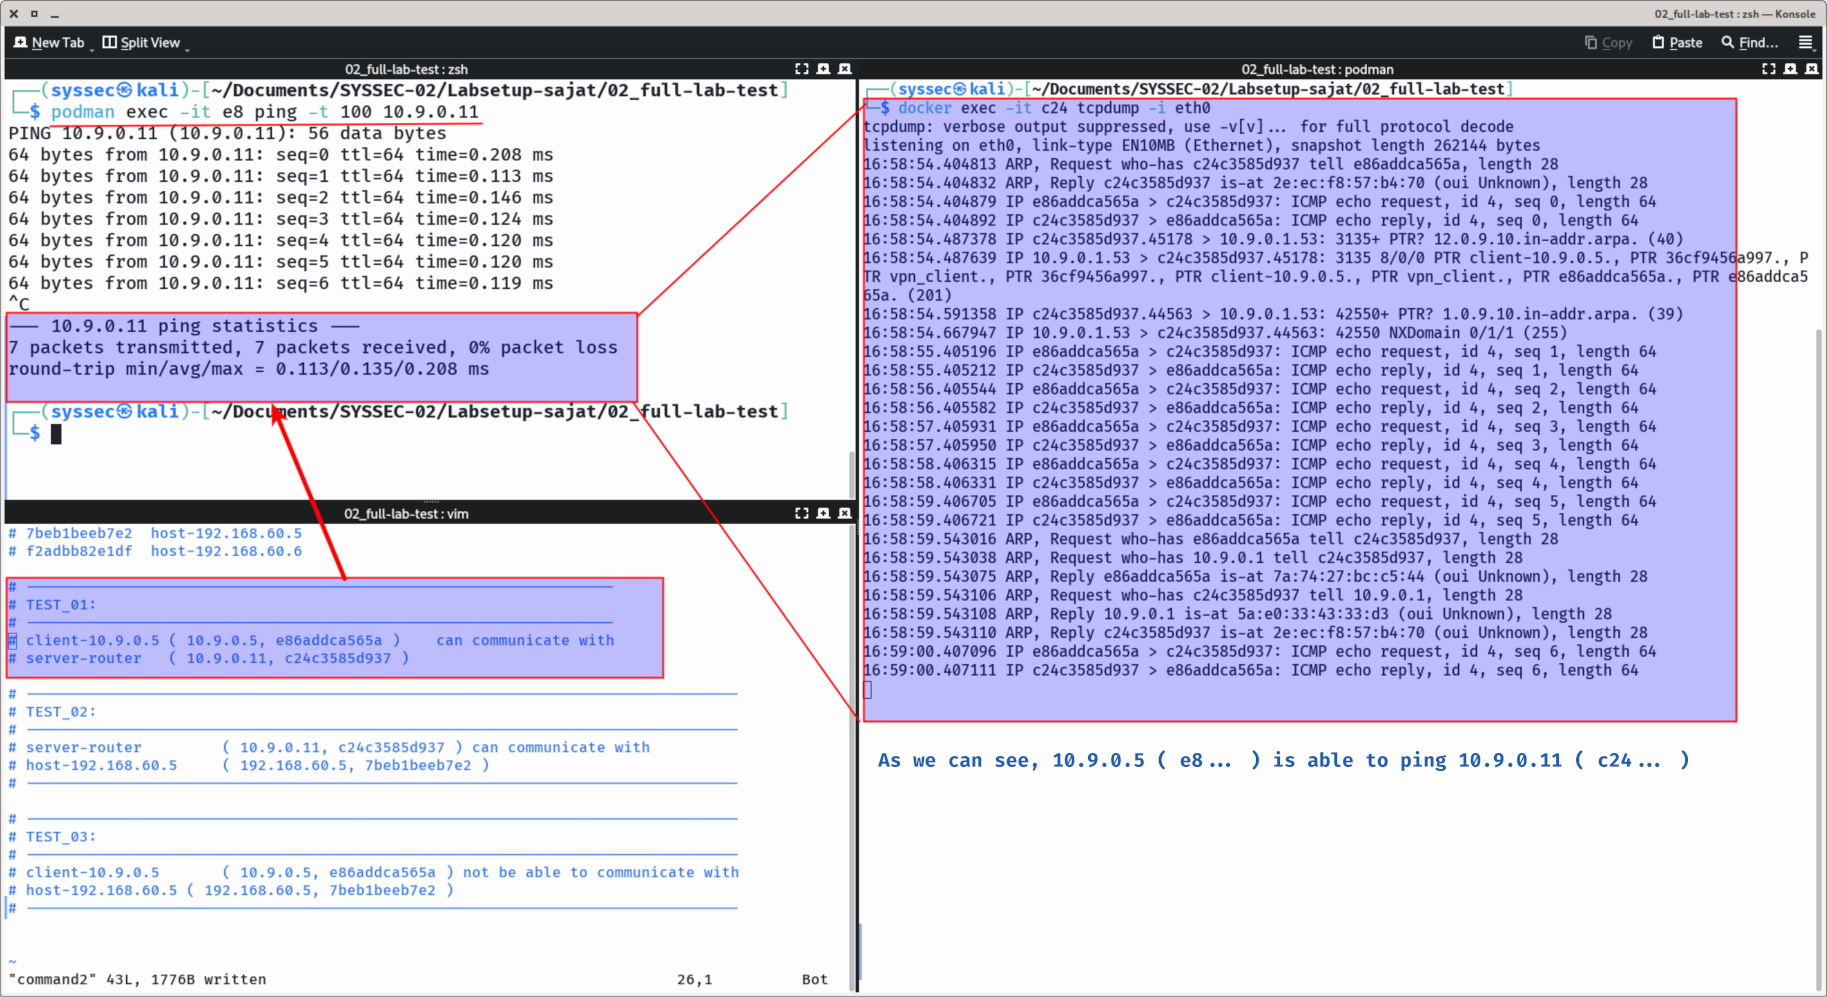
\includegraphics[width=0.5\linewidth]{Picture/02_Lab-exercises/020_connectivity-test/03_LAB-TEST__seed-01.pdf.png}
    \caption{ Host 192.168.50.5 (which also assigned to \textit{10.9.0.11}) can communicate with VPN Server}
    \label{fig:vpn-server-reach}
\end{figure}

Figure \ref{fig:site-b-reach} shows that VPN Server can communicate with \textit{Site B}:

\begin{figure}
    \centering
    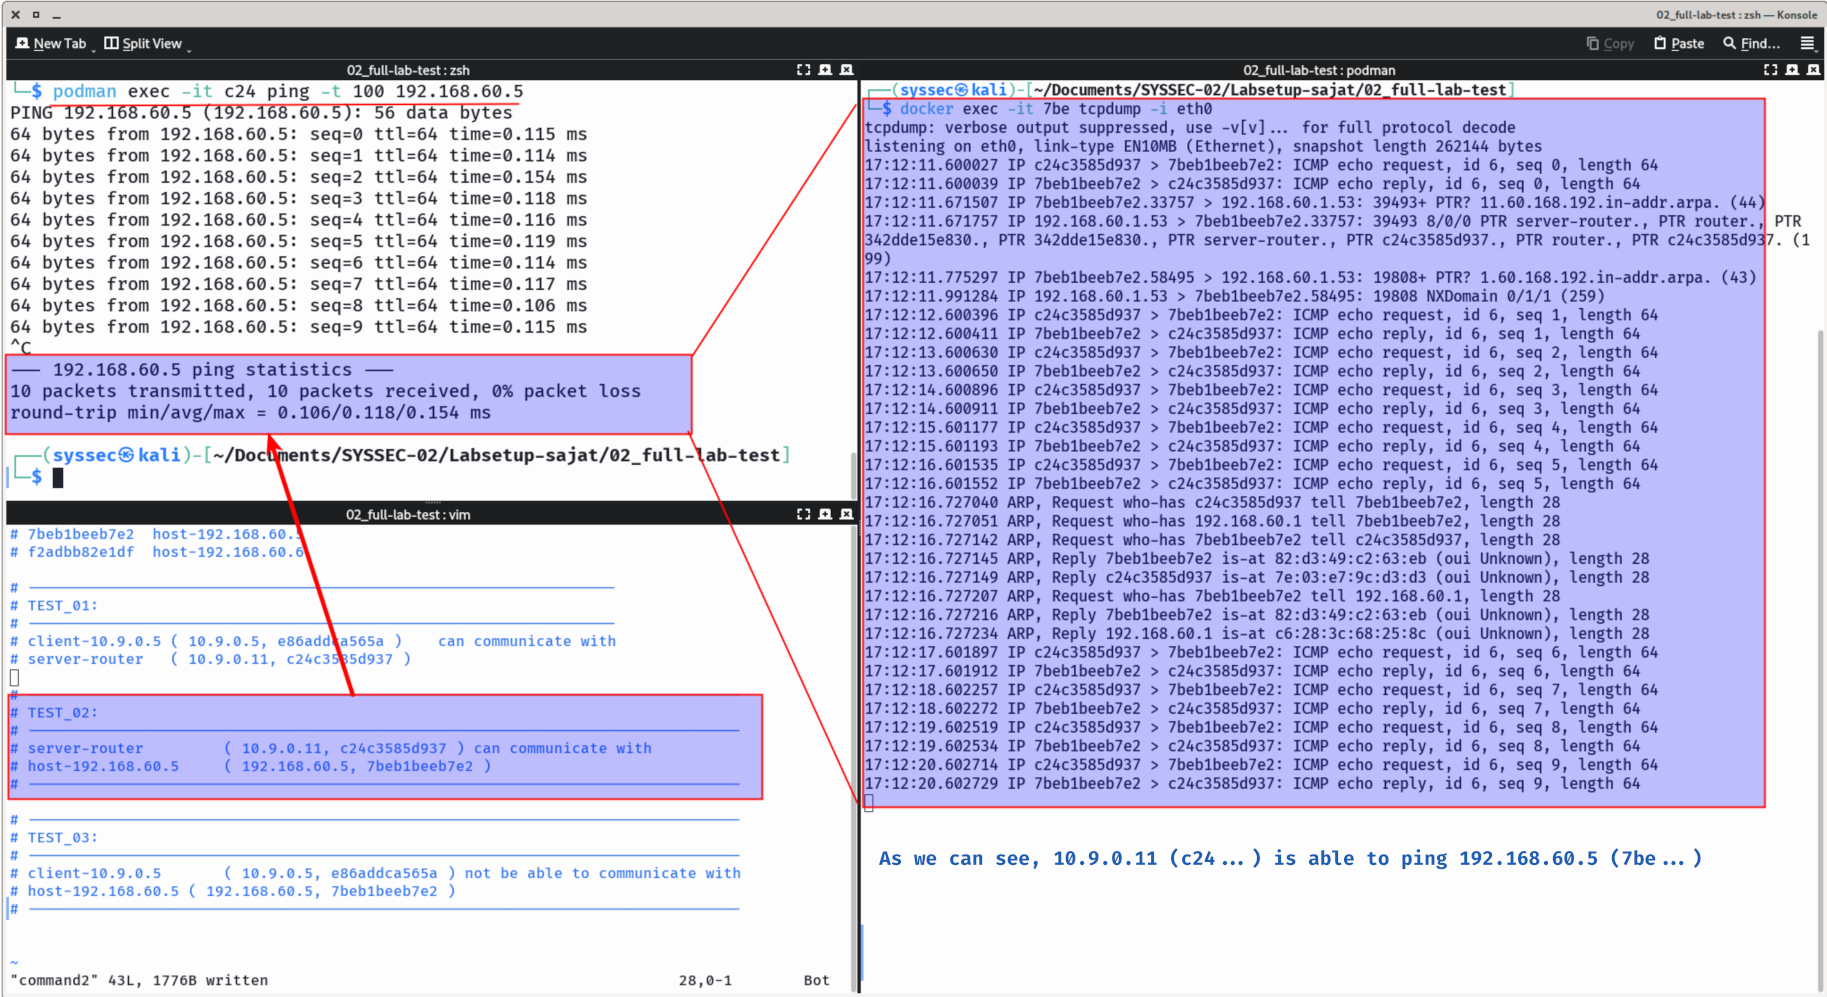
\includegraphics[width=0.65\linewidth]{Picture/02_Lab-exercises/020_connectivity-test/03_LAB-TEST__seed-02.pdf.png}
    \caption{ VPN Server can communicate with \textit{Site B}}
    \label{fig:site-b-reach}
\end{figure}

% tunnel
\section{Building blocks for the VPN tunnel}
\subsection{Configuring the TUN/TAP interface}

The VPN tunnel that we are going to build is based on the \textit{TUN/TAP} technologies. \textit{TUN} and \textit{TAP} are virtual network kernel drivers (please refer the code snippet below), they implement network device that are supported entirely in software. 

\textit{TAP} (as in network tap) simulates an Ethernet device and it operates with layer-2 packets such as \textit{Ethernet} frames, \textit{TUN} (as in network TUNnel) simulates a network layer device and it operates with layer-3 packets such as \textit{IP} packets. \cite{seedlab2024, libckernel}

With \textit{TUN/TAP}, we can create virtual network interfaces. A user-space program is usually attached to the TUN/TAP virtual network interface. Packets sent by an operating system via a TUN/TAP network interface are delivered to the user-space program.  \cite{seedlab2024, libckernel}

\begin{lstlisting}[language=python, caption=Creation of /dev/net/tun interface in Scapy]
# Create the `tun` interface
tun = os.open("/dev/net/tun", os.O_RDWR)
ifr = struct.pack('16sH', b'tun%d', IFF_TUN | IFF_NO_PI)
ifname_bytes  = fcntl.ioctl(tun, TUNSETIFF, ifr)
\end{lstlisting}

Packets sent by the program via a \textit{TUN/TAP} network interface are injected into the operating system network stack. To the operating system, it appears that the packets come from an external source through the virtual network interface.

When a program is attached to a \textit{TUN/TAP} interface, \textit{IP} packets sent by the kernel to this interface will be piped into the program. On the other hand, IP packets written to the interface by the program will be piped into the kernel, as if they came from the outside through this virtual network interface. The program can use the standard \lstinline{read()} and \lstinline{write()} system calls to receive packets from or send packets to the virtual interface.\cite{seedlab2024, libckernel}

The following code snippet showcases SeedLab's Task 2a.\cite{seedlab2024}.

\begin{lstlisting}[language=python, caption=Add an arbitrary name to tun0 interface]
# Create the tun interface
tun = os.open("/dev/net/tun", os.O_RDWR)
ifr = struct.pack('16sH', b'vadasz-tunnel%d', IFF_TUN | IFF_NO_PI)
ifname_bytes  = fcntl.ioctl(tun, TUNSETIFF, ifr)
\end{lstlisting}

With slightly modification the actual interface name can be changed as seen before. In the given task I changed it to \lstinline{vadasz-tunnel}, which can be seen on figure: 

\begin{figure}[h]
    \centering
    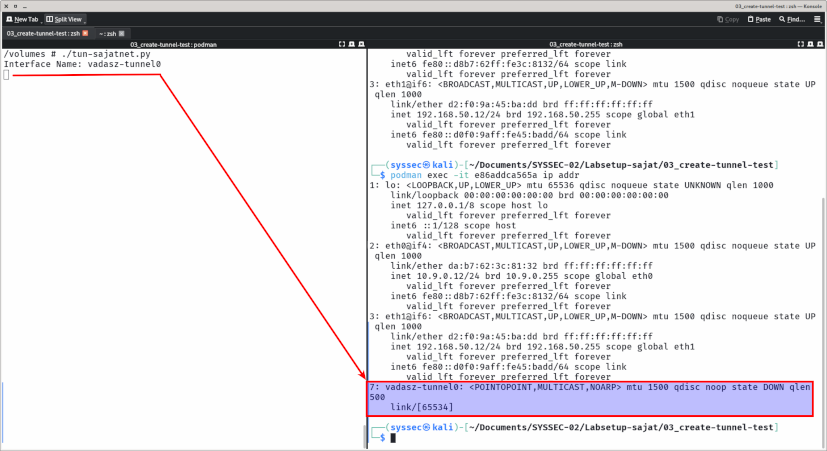
\includegraphics[width=0.65\linewidth]{Picture/02_Lab-exercises/01b_vadasztunnel0-interface.pdf.png}
    \caption{Renaming $/dev/net/tun$ interface name}
    \label{fig:enter-label}
\end{figure}

At this point, the \textit{TUN} interface is not usable, because it has not been configured yet. There are two things that we need to do before the interface can be used. 

First, we need to assign an IP address to it. Second, we need to bring up the interface, because the interface is still in the \textit{DOWN} state. The following code snippets shows how to bring up interface for \lstinline{tun0}, with mask \lstinline{/24}:

\begin{lstlisting}[language=python, caption=Change the state of TUN interface]
    # Equivalent to the command: ip addr add 192.168.53.99/24 dev tun0
    os.system("ip addr add 192.168.53.99/24 dev {}".format(ifname))
    # Equivalent to the command: ip link set dev tun0 up
    os.system("ip link set dev {} up".format(ifname))
    print("State changed to UP on interface: {}".format(ifname))
\end{lstlisting}

After changing the \lstinline{tun0} device's state to \lstinline{IP} we are able to reach the interface properly, showcased on \textit{figure \ref{fig:tun0up}}:

\begin{figure}[h]
    \centering
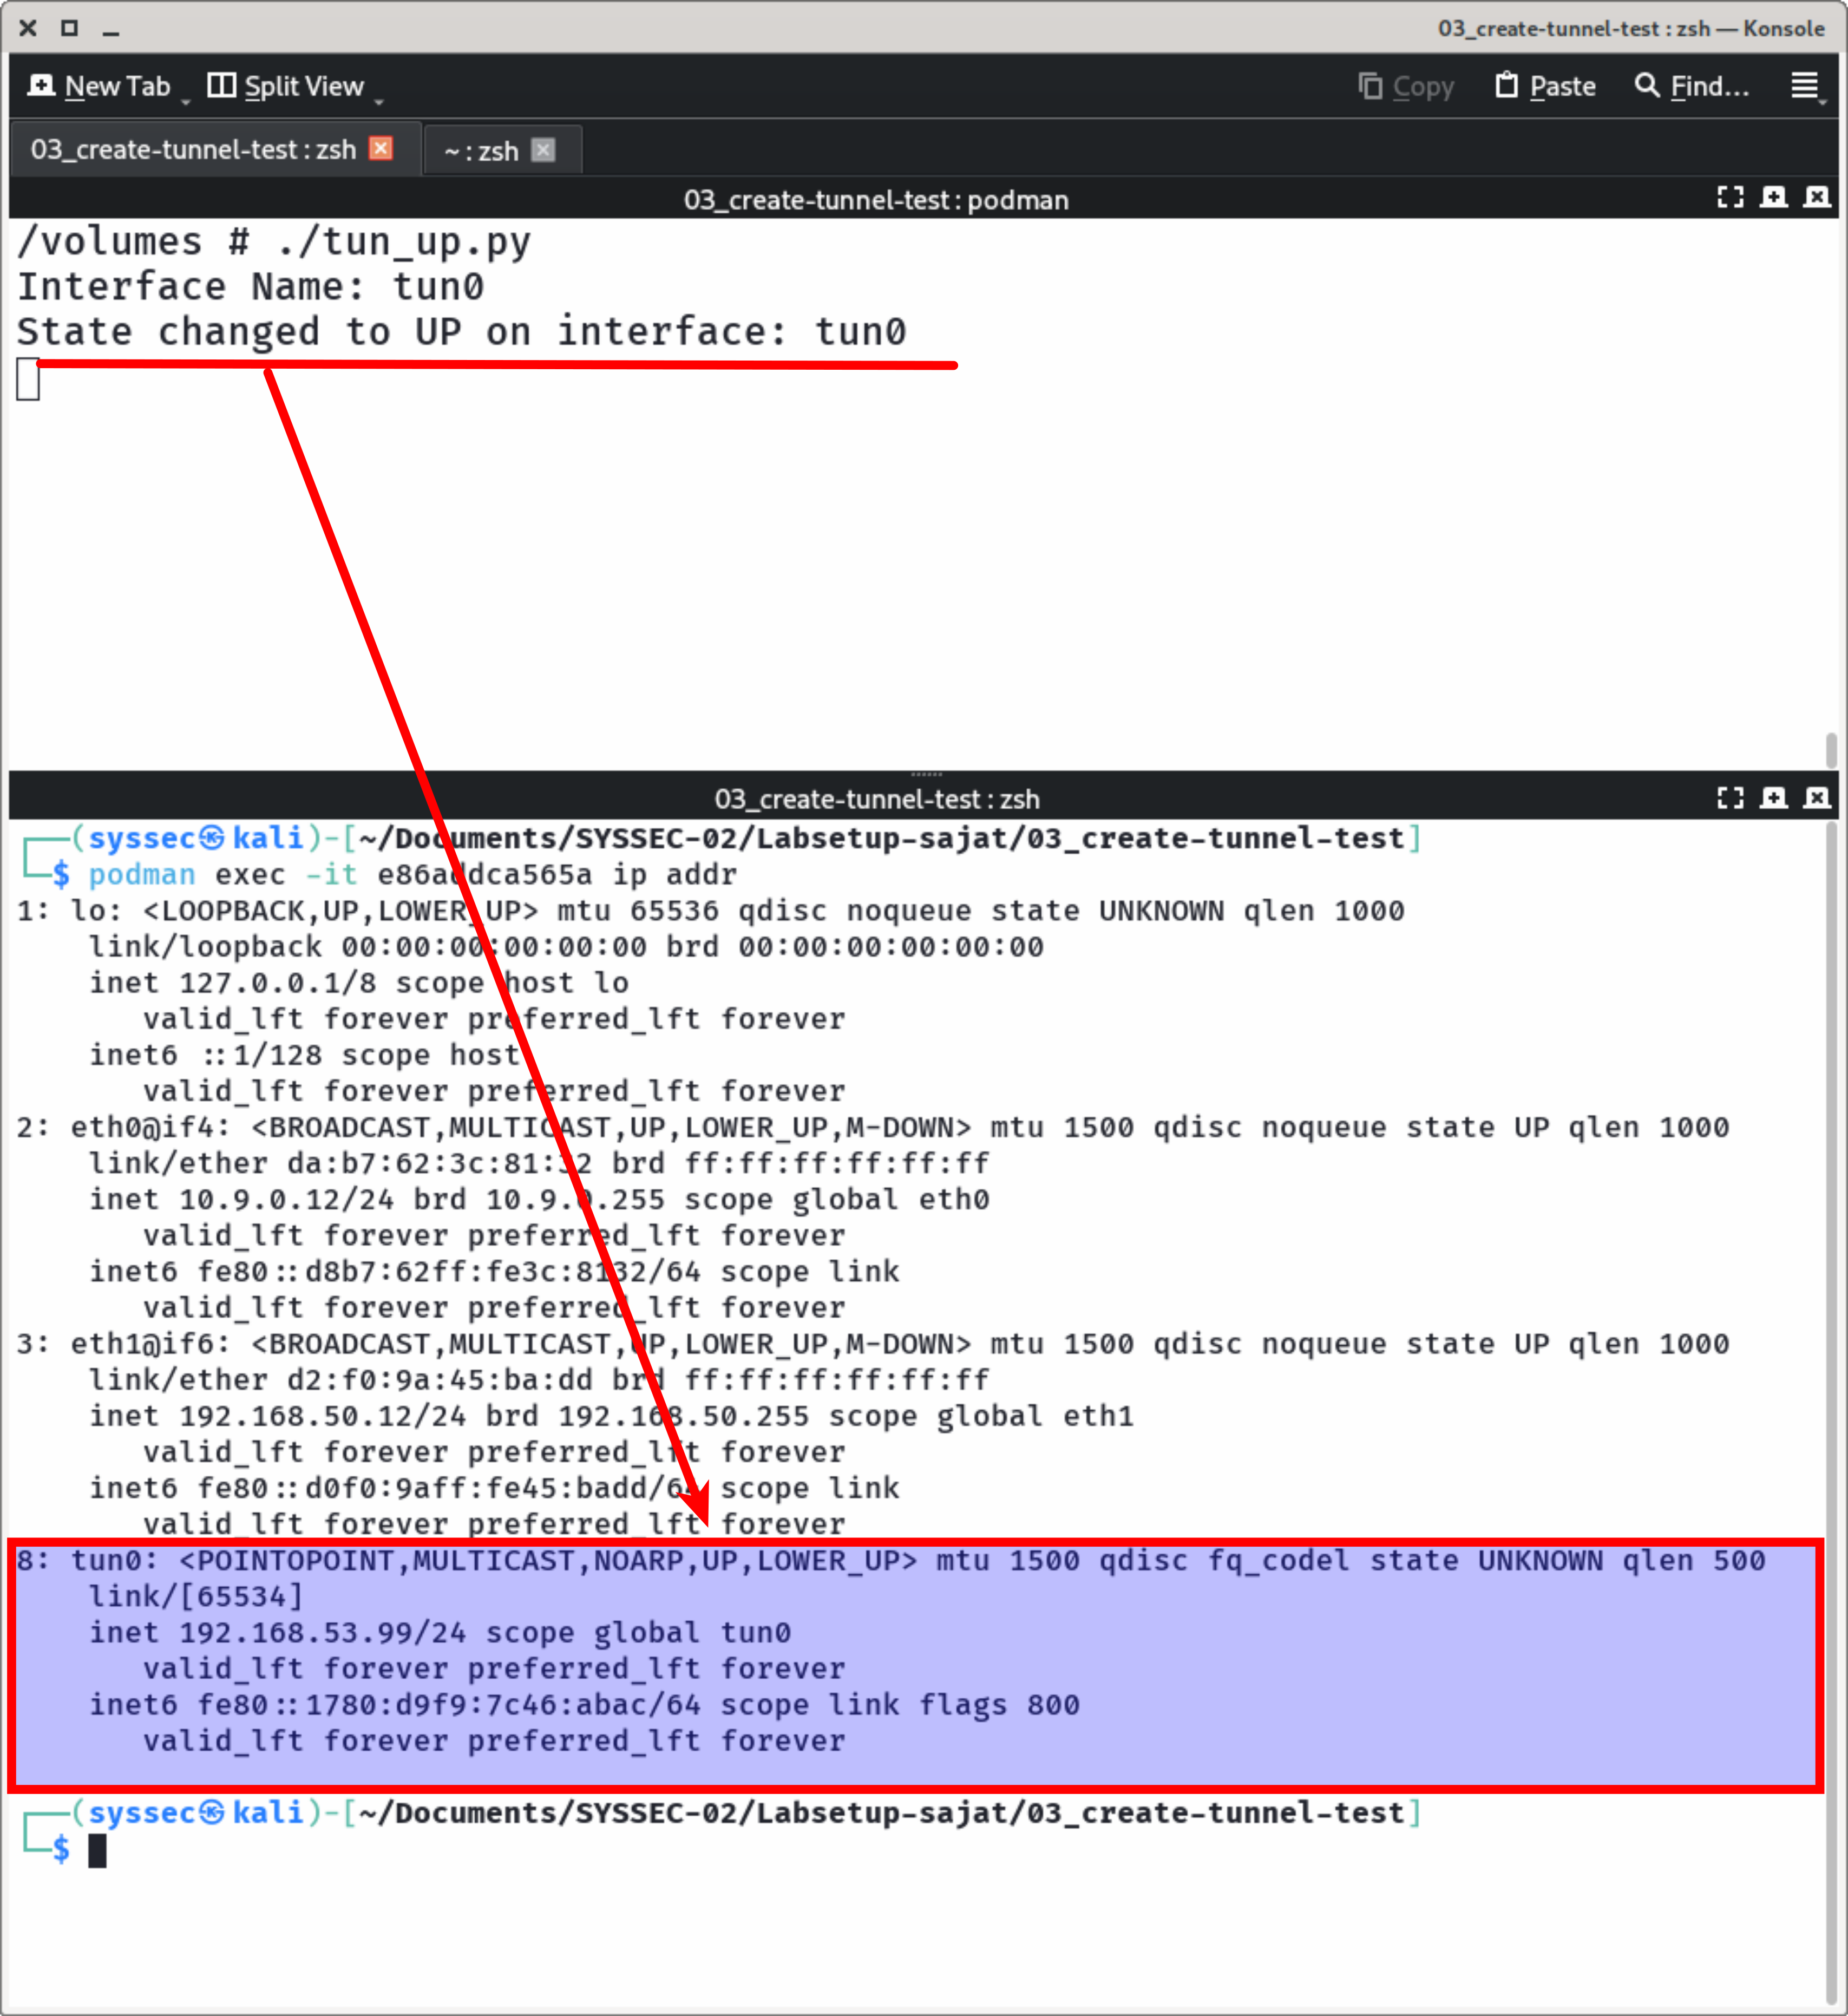
\includegraphics[width=0.45\linewidth]{Picture/02_Lab-exercises/02b_tun0-interface-UP.pdf.png}
    \caption{IP address assigned to interface \lstinline{tun0},  state changed from \lstinline{DOWN}}
    \label{fig:tun0up}
\end{figure}

\subsection{Read from TUN interface}

Now the interface \lstinline{tun0} is reachable, but to be able read from it I should cast the data received from the interface into a \textit{Scapy IP} object.\cite{seedlab2024}

The following code snippet from file \lstinline{02b_read-from-tunnel.py} showcases the modification: 

\begin{lstlisting}[language=python, caption=Reading IP packets from TUN interface]
# ==========================
# Reading from TUN interface
# ==========================

# Modifying `tun0.py` so we can read from the TUN interface.
# We can cast the data received from the interface
# into a scapy IP object, thus we can print out
# each field of the IP packet.

while True:
	# Get a packet from the `tun0` interface
	packet = os.read(tun,2048)
	if packet:
		ip = IP(packet)
		print(ip.summary())

\end{lstlisting}

Whatever coming out from the \lstinline{TUN} interface is an \textit{IP
packet}.
On \lstinline{VPN-CLIENT}, after I send out a ping to host (for the sake of example I choosed to ping a non existent host within the \lstinline{/24} subnet: \lstinline{192.168.53.1} ) in the \lstinline{192.168.53.0/24} network the program \lstinline{02b_read-from-tunnel.py} will read the ICMP echo request from the actual \lstinline{IPv4} address \lstinline{192.168.53.99/32} of the tunnel interface directly.
With the use of Scapy's layering capability regarding \lstinline{IP()} , I'm able to describe the incoming packets summary with \lstinline{ip.summary()} showcased on \textit{figure \ref{fig:02ctun0route}}:

\begin{figure}[h]
    \centering
    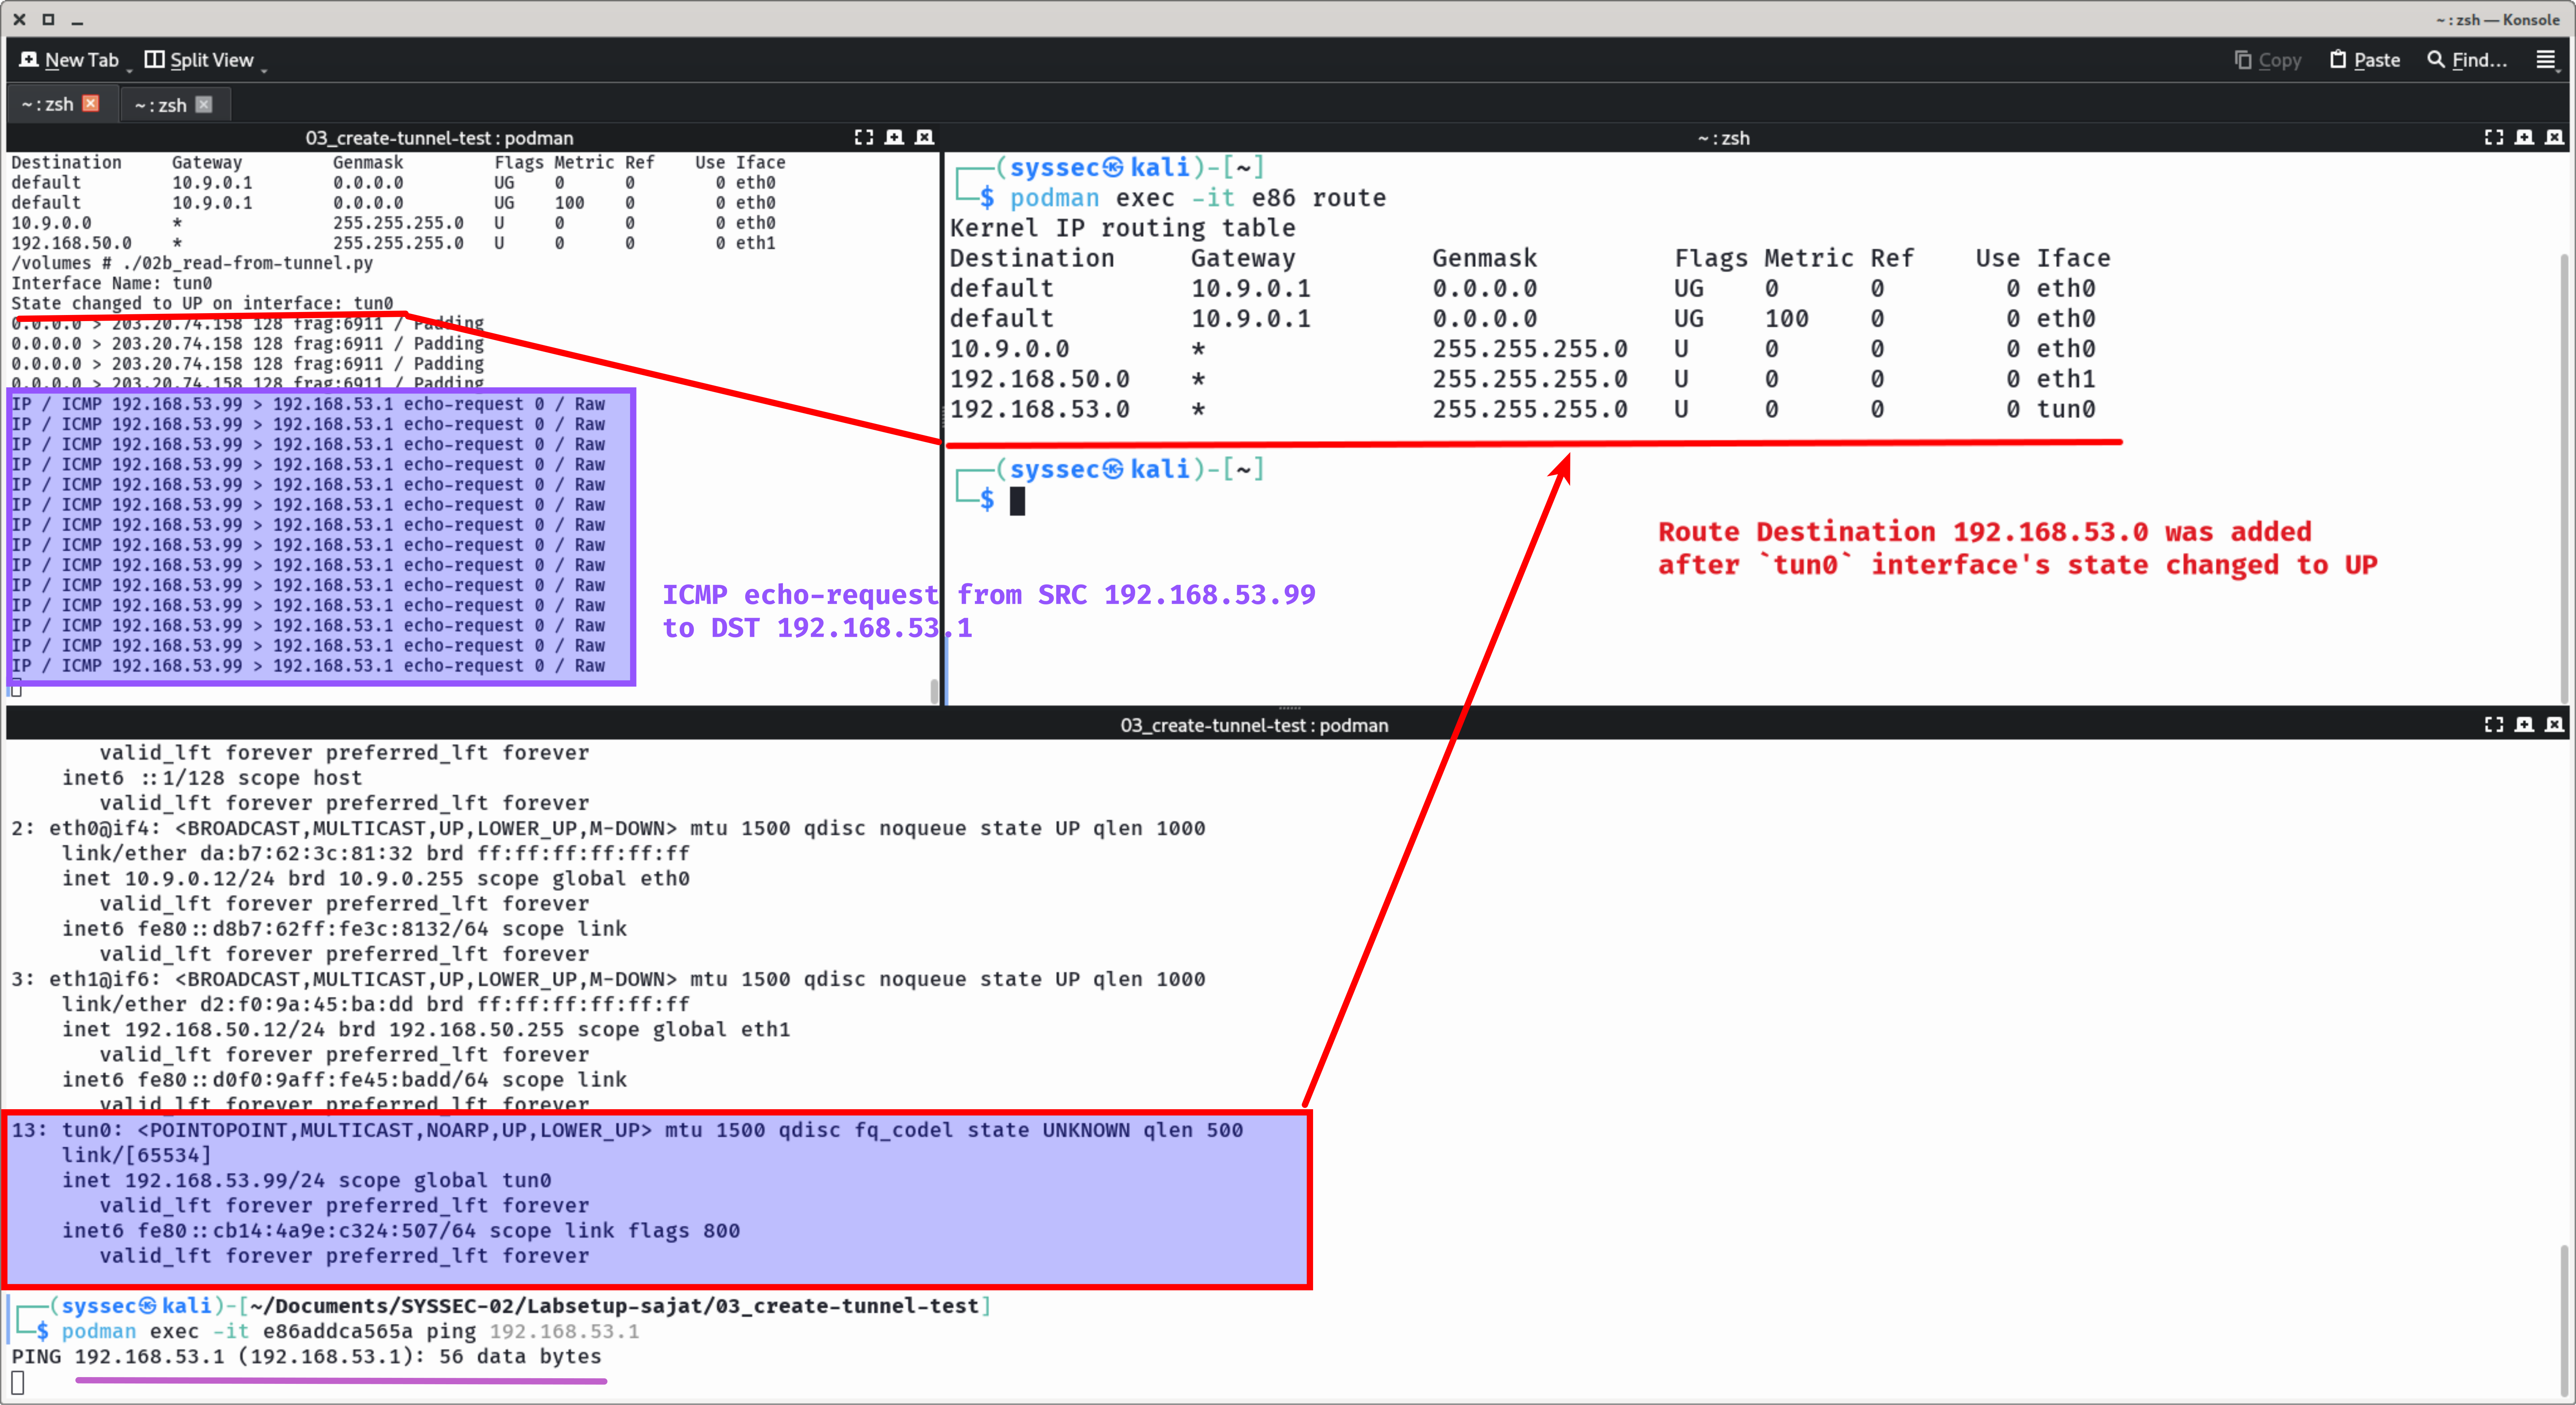
\includegraphics[width=0.65\linewidth]{Picture/02_Lab-exercises/02c_tun0-route.pdf.png}
    \caption{Reading ICMP echo request packets directly from \lstinline{tun0} interface }
    \label{fig:02ctun0route}
\end{figure}

Sending an \textit{ICMP echo request} to a host in the internal network of \lstinline{192.168.60.0/24}, will not print out anything anything, since as for now the \lstinline{tun0} interface is only configured on the host called \textit{VPN-Client} (\lstinline{192.168.50.12}, \lstinline{10.9.0.12}), In addict the correct routing through \lstinline{tun0} is missing currently in the file \lstinline{02b_read-from-tunnel.py}, thus the subnet \lstinline{192.168.60.0/24} is unreachable for now.

\subsection{Writing to TUN interface}

As for now I am able to read packets that are being sent to interface \lstinline{tun0}, furthermore I  will construct a new packet based on the received packet.

To do so I will need to modify \lstinline{02b_read-from-tunnel.py} as follows (please note the code snippet is from the file \lstinline{34a_read-and-write-to-tun.py}):

\begin{lstlisting}[language=python, caption=Reading ICMP packets from tun0 interface]
    # Read a packet from the `tun0` interface
    packet = os.read(tun, 2048)
    
    if packet:
        ip = IP(packet)
        
        # Check if it's an ICMP Echo Request (Type 8)
        if ip.haslayer(ICMP) and ip[ICMP].type == 8:
            print(f"Received ICMP Echo Request: {ip.summary()}")
\end{lstlisting}

After importing the necessary scapy modules with \lstinline{from scapy.all import *} I'm able to read a packet from \lstinline{tun0} with \lstinline{os.read(tun, 2048)}, 
with the condition \lstinline{ip.haslayer(ICMP) and ip[ICMP].type == 8} I'm able to tell wheter the IP packet has ICMP layer, and if so it is an ICMP echo request (\lstinline{type 8}) or response (\lstinline{type 0}) according to \lstinline{RFC 2780}, \lstinline{RFC 792} \cite{ianaicmpnumbers}.

For a more comprehensive use of \textit{Scapy} please refer to \textit{Appendix \ref{apx:icmp}}.

In case the packet is an ICMP echo request, then I construct the response to the
given packet as follows:

\begin{lstlisting}[language=python, caption=Create the corresponding ICMP echo reply with Scapy]
    # Create the corresponding ICMP Echo Reply (Type 0)
        icmp_reply = IP(src=ip.dst, dst=ip.src) / 
        ICMP(type=0, id=ip[ICMP].id, seq=ip[ICMP].seq) / 
        ip[ICMP].payload
\end{lstlisting}

After I set the sender's \textit{Source} and \textit{Destination} address values within the \textit{IPv4} header \cite{ipv4proto} \cite{ianaipv4proto} with \lstinline{IP(src=ip.dst, dst=ip.src)}, I construct the consequent ICMP response (\lstinline{type=0}) to the packet by read from \lstinline{tun0}. 

According to \cite{ianaicmpfields, ianaicmpnumbers} \textit{Identifier} (\lstinline{id=ip[ICMP].id}) and \textit{Sequence number} (\lstinline{seq=ip[ICMP].seq}) fields within the \lstinline{ICMP} header can be used by the client to match the reply with the request that caused the reply. For a more comprehensive use of \textit{Scapy} please refer to \textit{Appendix \ref{apx:icmp}}.
Lastly, I write back the response to \lstinline{tun0} interface using write method: \lstinline{os.write(tun, bytes(icmp_reply))}.

The \textit{Figure \ref{fig:readingandwritingtotun0}} showcases the case of successful reading of ICMP echo requests and writing back ICMP echo reponses  to \lstinline{tun0} interface:

\begin{figure}[h]
    \centering
    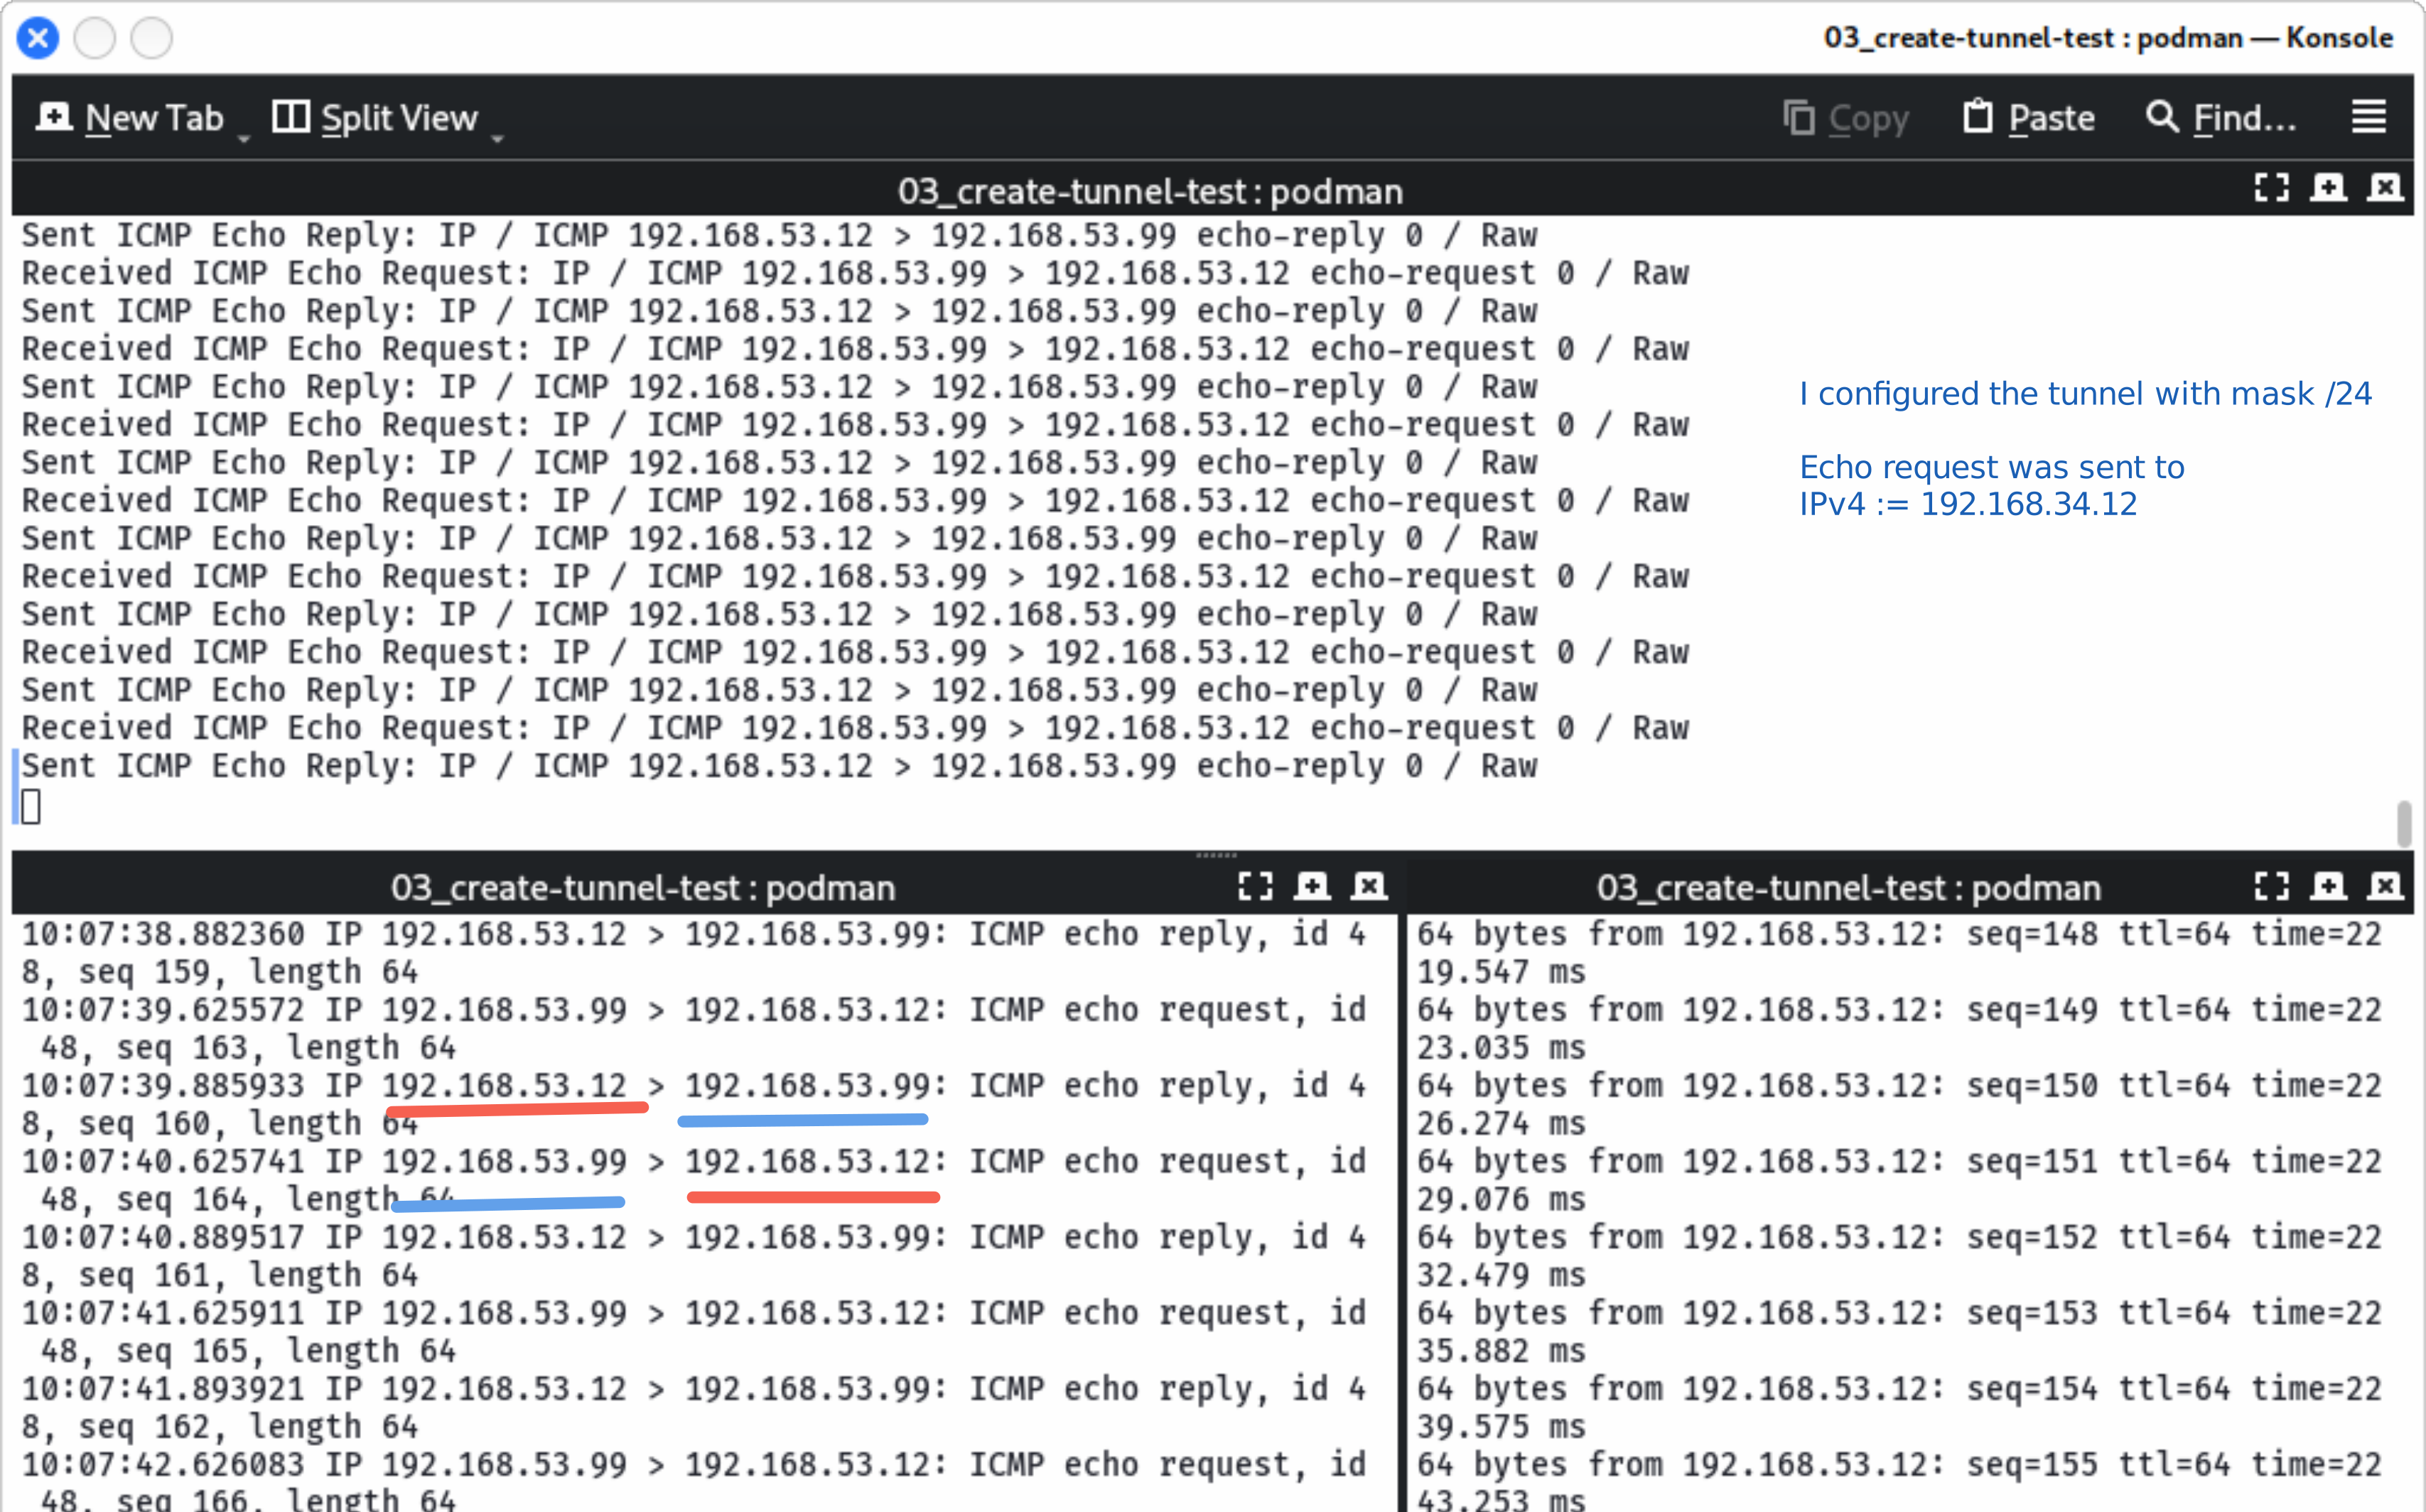
\includegraphics[width=0.65\linewidth]{Picture/02_Lab-exercises/34a_reading-and-writing-back-to__tun0-with-comments.pdf.png}
    \caption{Reading  and writing of \textit{ICMP} echo requests/responses  to \lstinline{tun0} interface}
    \label{fig:readingandwritingtotun0}
\end{figure}

After that, I modified the code to be able to  handle arbitrary data read and write from  \lstinline{tun0} as well. In the lab exercise I was asked to handle the case when I don't have \lstinline{IP()} layer. The problem is, that if I don't have the \lstinline{IP()} layer, I won't be able to write back \lstinline{IP} packets to given IP address, since ICMP "sits" on top of IP layer (by layer I mean here Scapy Layer).

To overcome this issue I crafted an arbitrary Scapy packet layering (please refer to file \lstinline{34b_read-and-write-to-tun-arbitrary-data.py})
structure \lstinline{Ethernet()/IP()/TCP()/custom_data} in mind (please refer to Figure \ref{fig:readwritearbtun0} )
as follows:

\begin{lstlisting}[language=python, caption=Write arbitrary data to tun0 interface]
# ....    
ether_packet = Ether(packet)	# Parse L2 layer into an Ether object
# ....    
    # Create a correspondig arbitrary data packet
    # Crafting with SourceMACField := 54:00:aa:bb:cc:ff
    # If we don't have IP() layer, use Ether() and  
    # layer 2 protocols instead
            custom_data = b"Random data on the wire !!"
            custom_ether=Ether(src="54:00:aa:bb:cc:ff",dst=ether_packet.src)
            custom_tcp=TCP(dport=443)/custom_data
            custom_ip=IP(src=ip.dst, dst="244.244.244.0")/custom_tcp         
\end{lstlisting}

First I parse the packet read from tunnel interface into an Scapy Ethernet object with \lstinline{Ether(packet)}. 
Secondly, for the response I made up the Ethernet layer (\lstinline{Ether()}) with  the source MAC address of \lstinline{54:00:aa:bb:cc:ff} with the destination MAC address of the sender (\lstinline{Ether(dst=ether_packet.src)}). 

Thirdly, I forged a customized IP packet with \lstinline{IP()}, with the destination IP Address of \lstinline{244.244.244.0}. (I choosed this IP address simply for the sake of presentation, from the actual lab experiment point of view, this IP address would be irrelevant since I want to send packets to Site B's subnet not outside of it.)

\begin{figure}[h]
    \centering
    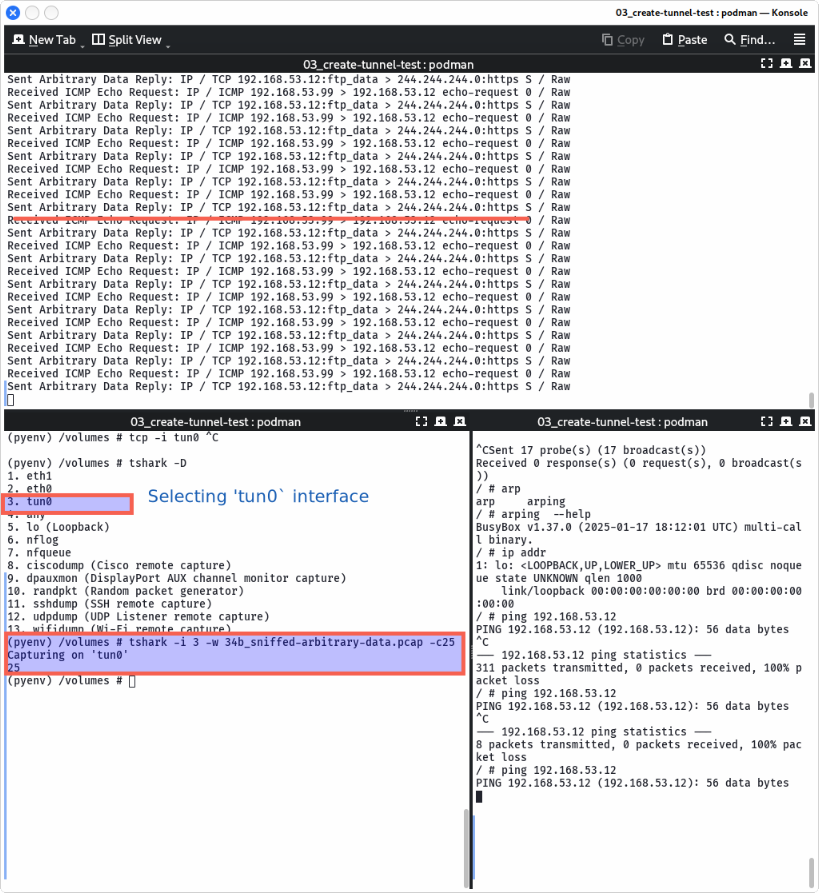
\includegraphics[width=0.45\linewidth]{Picture/02_Lab-exercises/34b_reading-and-writing-back-to__tun0-arbitrary-data-with-manual-ip.pdf.png}
    \caption{Sniffing the unencrypted arbitrary data on wrote back to interface \lstinline{tun0}}
    \label{fig:readwritearbtun0}
\end{figure}

Since \lstinline{34b_read-and-write-to-tun-arbitrary-data.py} file is a slightly modification of \lstinline{02b_read-from-tunnel.py} I didn't allocated a new variable for the IP object, thus I used the IP destination address from \lstinline{ip} object: \lstinline{icmp_reply = IP(src=ip.dst, dst=ip.src) / ...}. For the \lstinline{TCP} destination port I choosed \lstinline{443} on purpose, since this is the allocated port for https communication according to  RFC 1700 (obsoleted by: RFC 3232). \cite{allocatednumbers}. On the otherhand since I'm sending the packets unencrypted on the wire, I'll be able watch the unencrypted traffic (please refer to \textit{Figure \ref{fig:sniffarb}} ) by tapping into \lstinline{tun0} with \lstinline{tshark} using the following snippet:

\begin{lstlisting}[language=bash, caption=Sniffing unencrypted arbitrary data sent trough tun0 interface ]
# Check available interfaces 
tskark -D

# Select `tun0` interface and sniff 25 packets, 
# than write it to a pcap file
tshark -i 3 -w 34b_sniffed-arbitrary-data.pcap -c25
\end{lstlisting}

\begin{figure}[h]
    \centering
    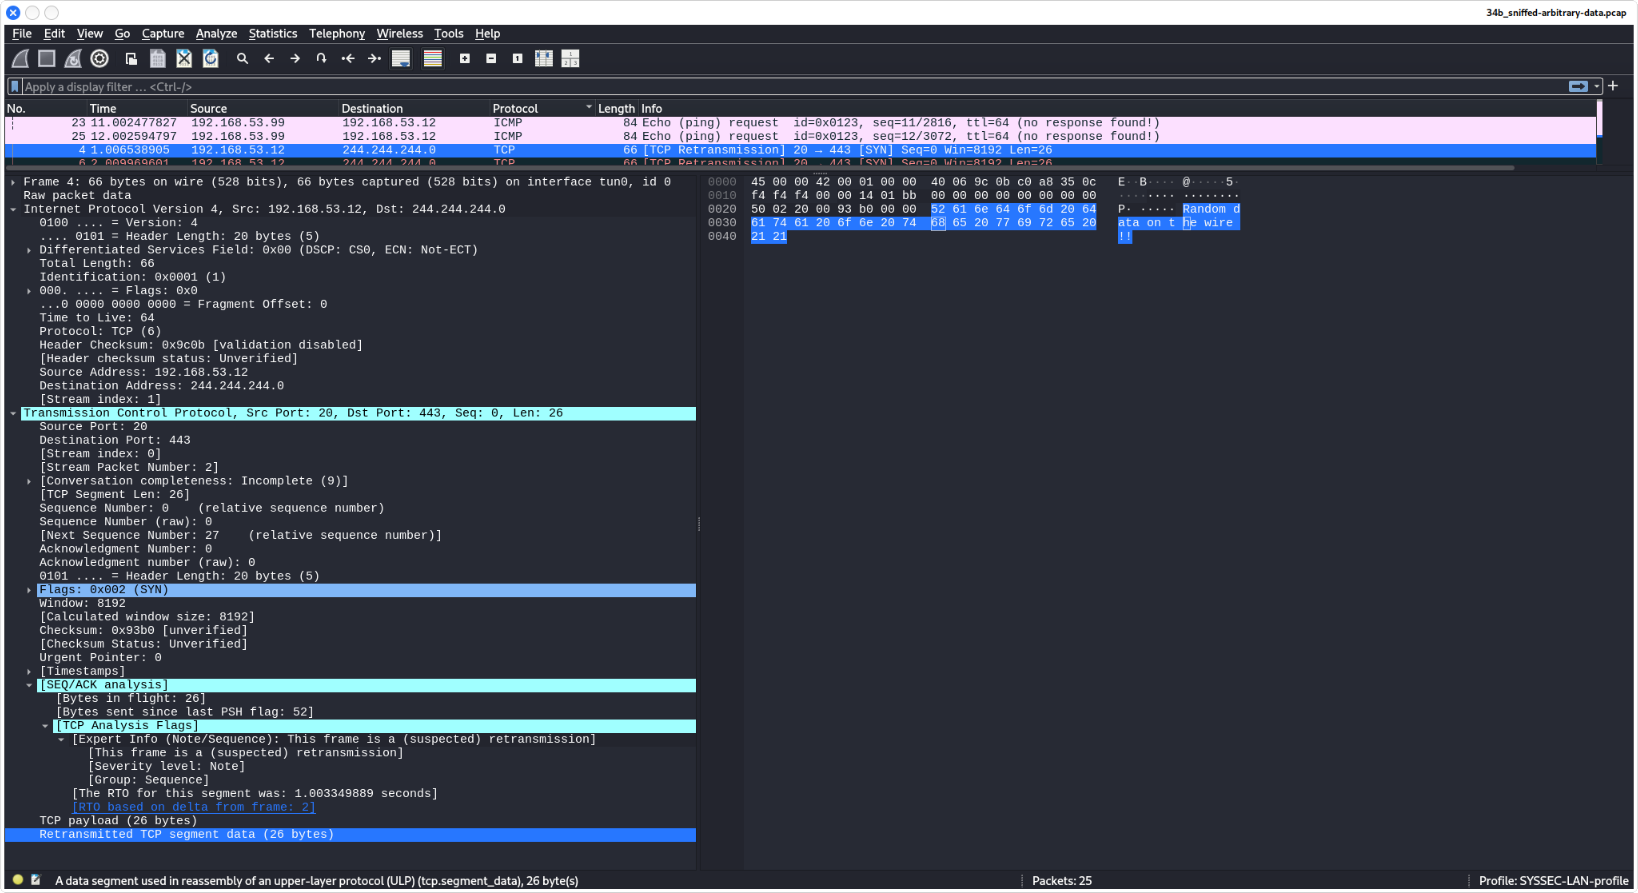
\includegraphics[width=0.65\linewidth]{Picture/02_Lab-exercises/34b_sniffed-arbitrary-data.pcap_001.pdf.png}
    \caption{Analyzing the captured unencrypted data from interface \lstinline{tun0} with \textit{wireshark}\cite{wiresharkorg} }
    \label{fig:sniffarb}
\end{figure}

For a more comprehensive use of \textit{Scapy} \lstinline{Ether()}, \lstinline{IP()}, \lstinline{TCP()} please refer to \textit{Appendix \ref{apx:ethernet}, \ref{apx:ipv4}, \ref{apx:tcp}}. On the right hand side the unencrypted traffic sent over \lstinline{tun0} becomes readable showcased on \textit{Figure \ref{fig:arbitdatawire}}:

\begin{figure}
    \centering
    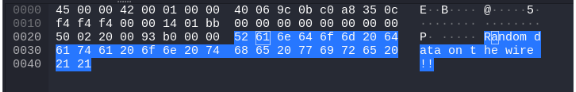
\includegraphics[width=0.65\linewidth]{Picture/02_Lab-exercises/34b_sniffed-arbitrary-data.pcap.pdf.png}
    \caption{Reading arbitrary data \lstinline{Random data on the wire !!} on the \lstinline{tun0}}
    \label{fig:arbitdatawire}
\end{figure}


\subsection{Sending IP packets to VPN server trough a tunnel}
\label{ssec:tunnl.send}



Next I will put the IP packet received from the \lstinline{tun0} interface into the TCP payload field of a new IP packet, and send it to another computer. Namely, I place the original packet inside a new packet. This
is called IP tunneling. \cite{seedlab2024}

The following snippets shows the tcp server (please refer to \lstinline{04_tun-server.py}) running on host \lstinline{VPN-Server} (\lstinline{192.168.60.11}, \lstinline{10.9.0.11}).

\begin{lstlisting}[language=python, caption=TCP Server test]
IP_A = "0.0.0.0"
PORT = 9090

# Create a TCP socket
sock = socket.socket(socket.AF_INET, socket.SOCK_STREAM)
sock.bind((IP_A, PORT))

\end{lstlisting}

The server is listening on port \lstinline{9090} and prints out whatever is receives. The program assumes that the data in the TCP payload field is an IP packet, so it casts the payload to a Scapy IP object, thus it prints out the source and destination IP address of the enclosed IP packet as can be seen on \textit{Figure \ref{fig:pingtestvpnserver}}. 

\begin{figure}[h]
    \centering
    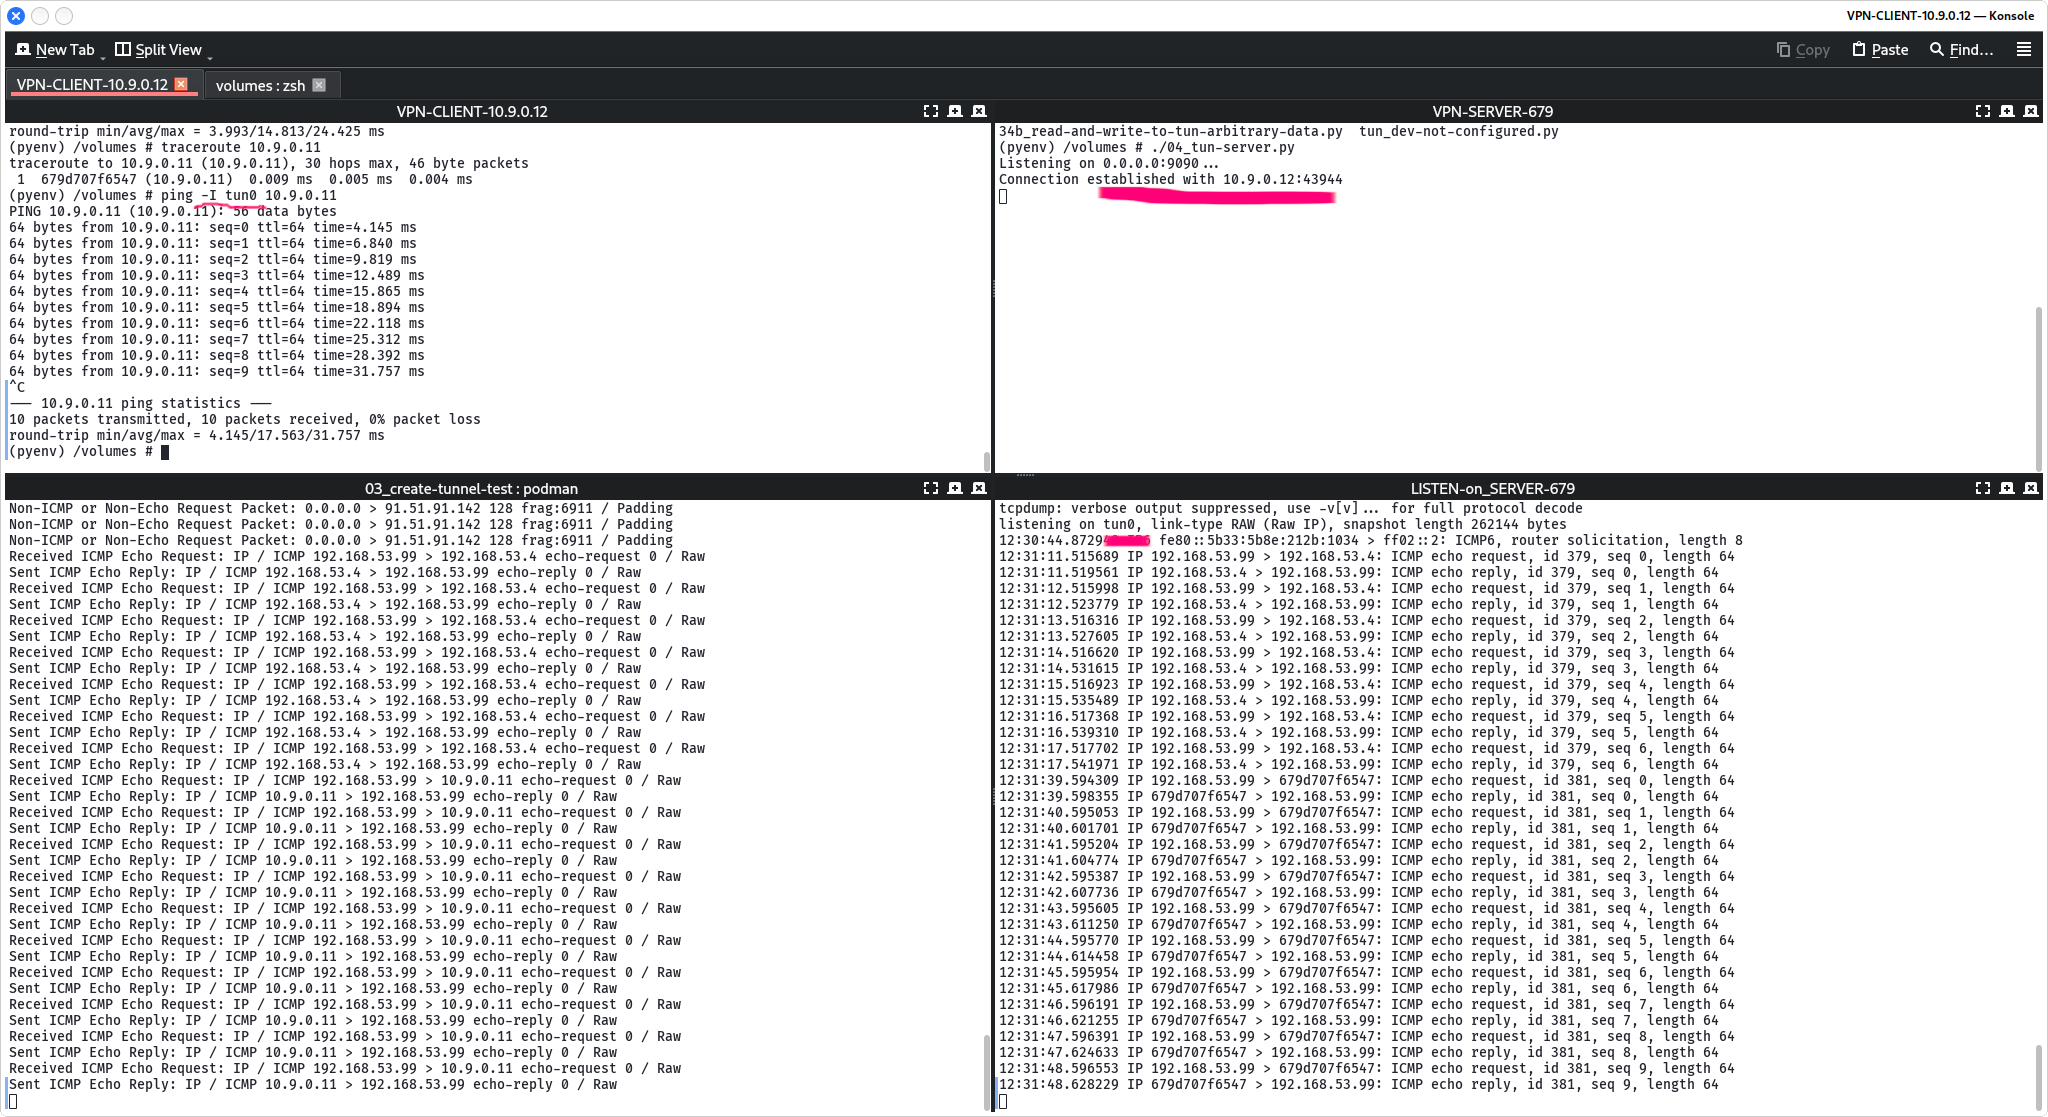
\includegraphics[width=0.65\linewidth]{Picture/03_lab-exercise-tunnel/04-ping-server-from-tun0-on-client.png.png}
    \caption{Sending ICMP echo request explicitly  on \lstinline{tun0} from \textit{VPN client} to \textit{VPN server}: \lstinline{ping -I tun0 10.9.0.11}}
    \label{fig:pingtestvpnserver}
\end{figure}

To be able to reach hosts from \lstinline{192.168.50.0/24} range I'll add the route with \lstinline{ip route add 192.168.60.99/24 dev tun0 via 10.9.0.11}. Now the packets will routed to the TUN interface, to test that I pinged the \textit{VPN-Server} explicitly trough the tunnel interface with \lstinline{ping -I tun0 10.9.0.11}. Up until this point I'm able to reach the VPN-Server from subnet \lstinline{192.168.50.5/24}, but to be able to ping for example the host \lstinline{192.168.60.5} from \textit{Site B}, I need to enable IP forwarding on the host \textit{VPN-Server}. IP forwarding has already been enabled on the \textit{VPN-Server} container with \lstinline{net.ipv4.ip_forward=1}  please refer to \ref{apx:lab__building-the-complete-lab-environment} for the complete setup.

After \textit{VPN-Server} gets a packet from the tunnel, it needs to feed the packet to the kernel, so the kernel can route the packet towards its final destination as can be seen on \textit{Figure \ref{fig:pingsiteb}}. After getting to this point, one direction of the tunnel is complete, i.e., we can send packets from \lstinline{192.168.50.12}
to \lstinline{192.168.60.5} via the tunnel. If we look at the Wireshark trace on host \lstinline{192.168.60.5}, we can see that \lstinline{192.168.60.5} has sent out the response, but the packet gets dropped somewhere.  This is because our tunnel is only one directional; we need to set up its other direction, so returning traffic can be tunneled back to Host \lstinline{192.168.50.12}.\cite{seedlab2024}
To achieve that, our TUN client and server programs need to read data from two interfaces, the TUN interface and the socket interface.


\begin{figure}[h]
    \centering
    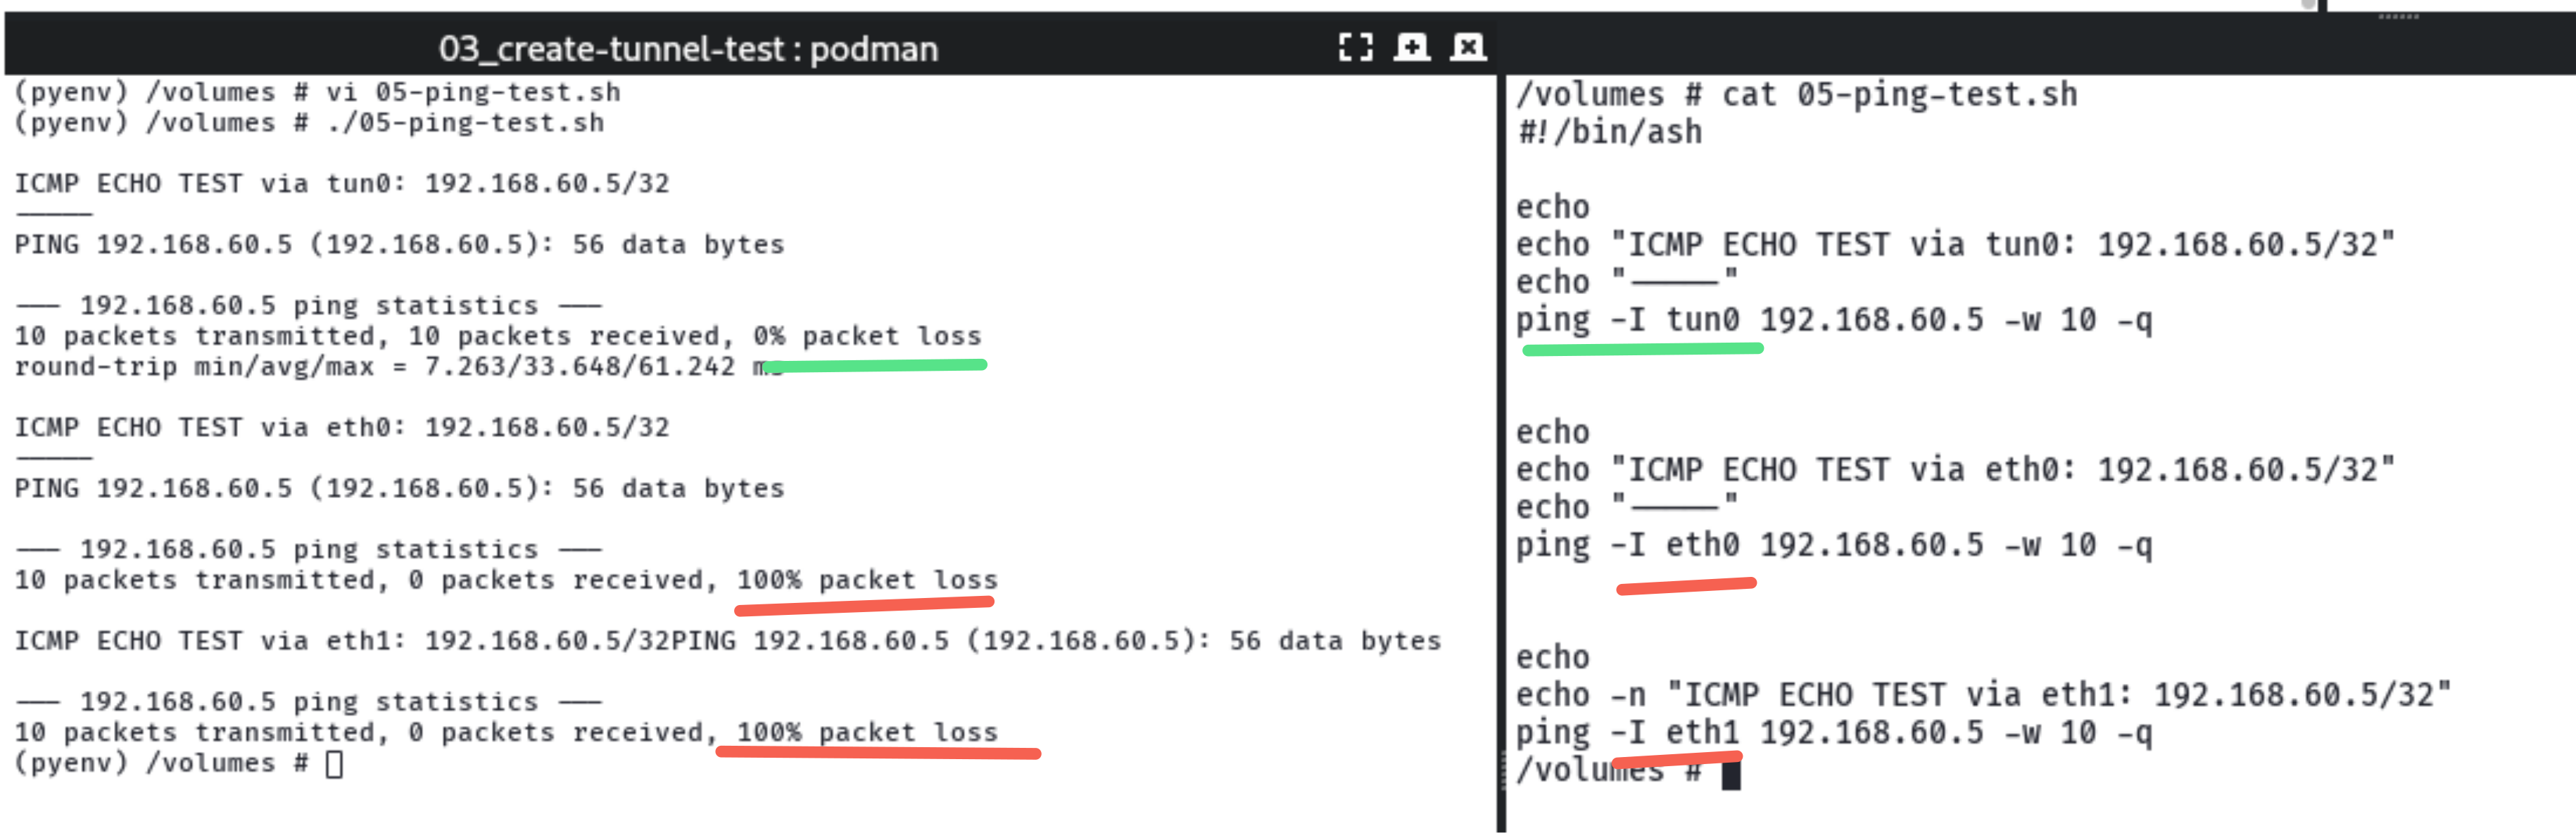
\includegraphics[width=0.65\linewidth]{Picture/03_lab-exercise-tunnel/05-host-echo-test.pdf.png}
    \caption{ICMP echo request sent to Site B host from Site A trough VPN tunnel trough interface \lstinline{tun0}}
    \label{fig:pingsiteb}
\end{figure}

All these interfaces are represented by file descriptors, so we need to monitor them to see whether there are data coming from them. One way to do that is to keep polling them,and see whether there are data on each of the interfaces. The performance of this approach is undesirable, because the process has to keep running in an idle loop when there is no data. Another way is to read from an interface. By default, read is blocking, i.e., the process will be suspended if there are no data. When data become available, the process will be unblocked, and its execution will continue. This way, it does not waste CPU time when there is no data.\cite{seedlab2024}


\subsection{Traffic Handling in both direction}

For one direction of your tunnel is complete, i.e., I can send packets from host \lstinline{192.168.50.12} to \lstinline{10.9.0.11} via the tunnel. Listening on \lstinline{tun0} \lstinline{10.9.0.11}, we can see that \lstinline{10.9.0.11} has sent out the response, but the packet gets dropped somewhere. This is because our tunnel is only one directional; I
need to set up its other direction, so returning traffic can be tunneled back to host \lstinline{192.168.50.12}.\cite{seedlab2024}

To achieve that, our TUN client and server programs need to read data from two interfaces, the TUN interface and the socket interface. All these interfaces are represented by file descriptors, so we need to monitor them to see whether there are data coming from them. One way to do that is to keep polling them, and see whether there are data on each of the interfaces. The performance of this approach is undesirable, because the process has to keep running in an idle loop when there is no data. \cite{seedlab2024}

Another way is to read from an interface. By default, read is blocking, i.e., the process will be suspended if there are no data. When data become available, the process will be unblocked, and its execution will continue. This way, it does not waste CPU time when there is no data. \cite{seedlab2024}

The read-based blocking mechanism works well for one interface. If a process is waiting on multiple interfaces, it cannot block on just one of the interfaces. It has to block on all of them altogether. Linux has a
system call called \lstinline{select()}, which allows a program to monitor multiple file descriptors simultaneously. To use \lstinline{select()}, I need to store all the file descriptors to be monitored in a set, and then we give the set to the \lstinline{select()} system call, which will block the process until data are available on one of the file descriptors in the set. 

In the following Python code snippet, I use \lstinline{select()} to monitor a TUN and a socket file descriptor: 

\begin{lstlisting}[language=python, caption=Handling bi-directional traffic  with \textit{Scapy}]
# ...
while True:
    # Use select to wait for the socket or tun to be ready
    ready, _, _ = select.select([tls_client.socket, tun], [], [])

    for fd in ready:
        if fd is tls_client.socket:
            try:
                # Read data from the TLS server
                data = tls_client.recv(2048)
                if data:
                    pkt = IP(data)
                    print("From TLS server <==: {} --> {}".format(pkt.src, pkt.dst))

                    # Forward packet to TUN interface
                    os.write(tun, bytes(pkt))  # Send data back to the TUN interface
                    print(f"Forwarded packet to TUN: {pkt.summary()}")

            except socket.error as e:
                print(f"Error reading from socket: {e}")

        if fd is tun:
            # Read a packet from the TUN interface
            packet = os.read(tun, 2048)
            if packet:
                pkt = IP(packet)
                print("From tun ==>: {} --> {}".format(pkt.src, pkt.dst))

                # Check if it's an ICMP Echo Request (Type 8)
                if pkt.haslayer(ICMP) and pkt[ICMP].type == 8:  # Type 8 is ICMP Echo Request
                    print(f"Received ICMP Echo Request: {pkt.summary()}")

# ...
\end{lstlisting}

After I add the routes through \lstinline{tun0} tunnel interface with the command \lstinline{ip route add 192.168.50.0/24 dev tun0}, I will be able to ping \textit{Site A}'s subnet (\lstinline{192.168.50.0/24}) as well from \textit{Site B} (\lstinline{192.168.60.0/24}). 

The following codesnippet showcases the routing table (the output of \lstinline{ip route} command) of host \textit{VPN-SERVER} (\lstinline{192.168.60.11}, \lstinline{10.9.0.11})

\begin{lstlisting}[language=bash,caption=Define static routes between Sites]
#  Route to subnet 192.168.50.0/24 successfully added via tun0
192.168.50.0/24 dev tun0 scope link 
#  tun0 interface successfully configured 
192.168.53.0/24 dev tun0 scope link  src 192.168.53.99 
\end{lstlisting}

Figure shows the case of successfully sent echo request with the command \lstinline{ping -I tun0 192.168.50.12} to host \lstinline{192.168.50.12} from \lstinline{192.168.60.12}  trough the interface \lstinline{tun0}: 

\begin{figure}[h]
    \centering
    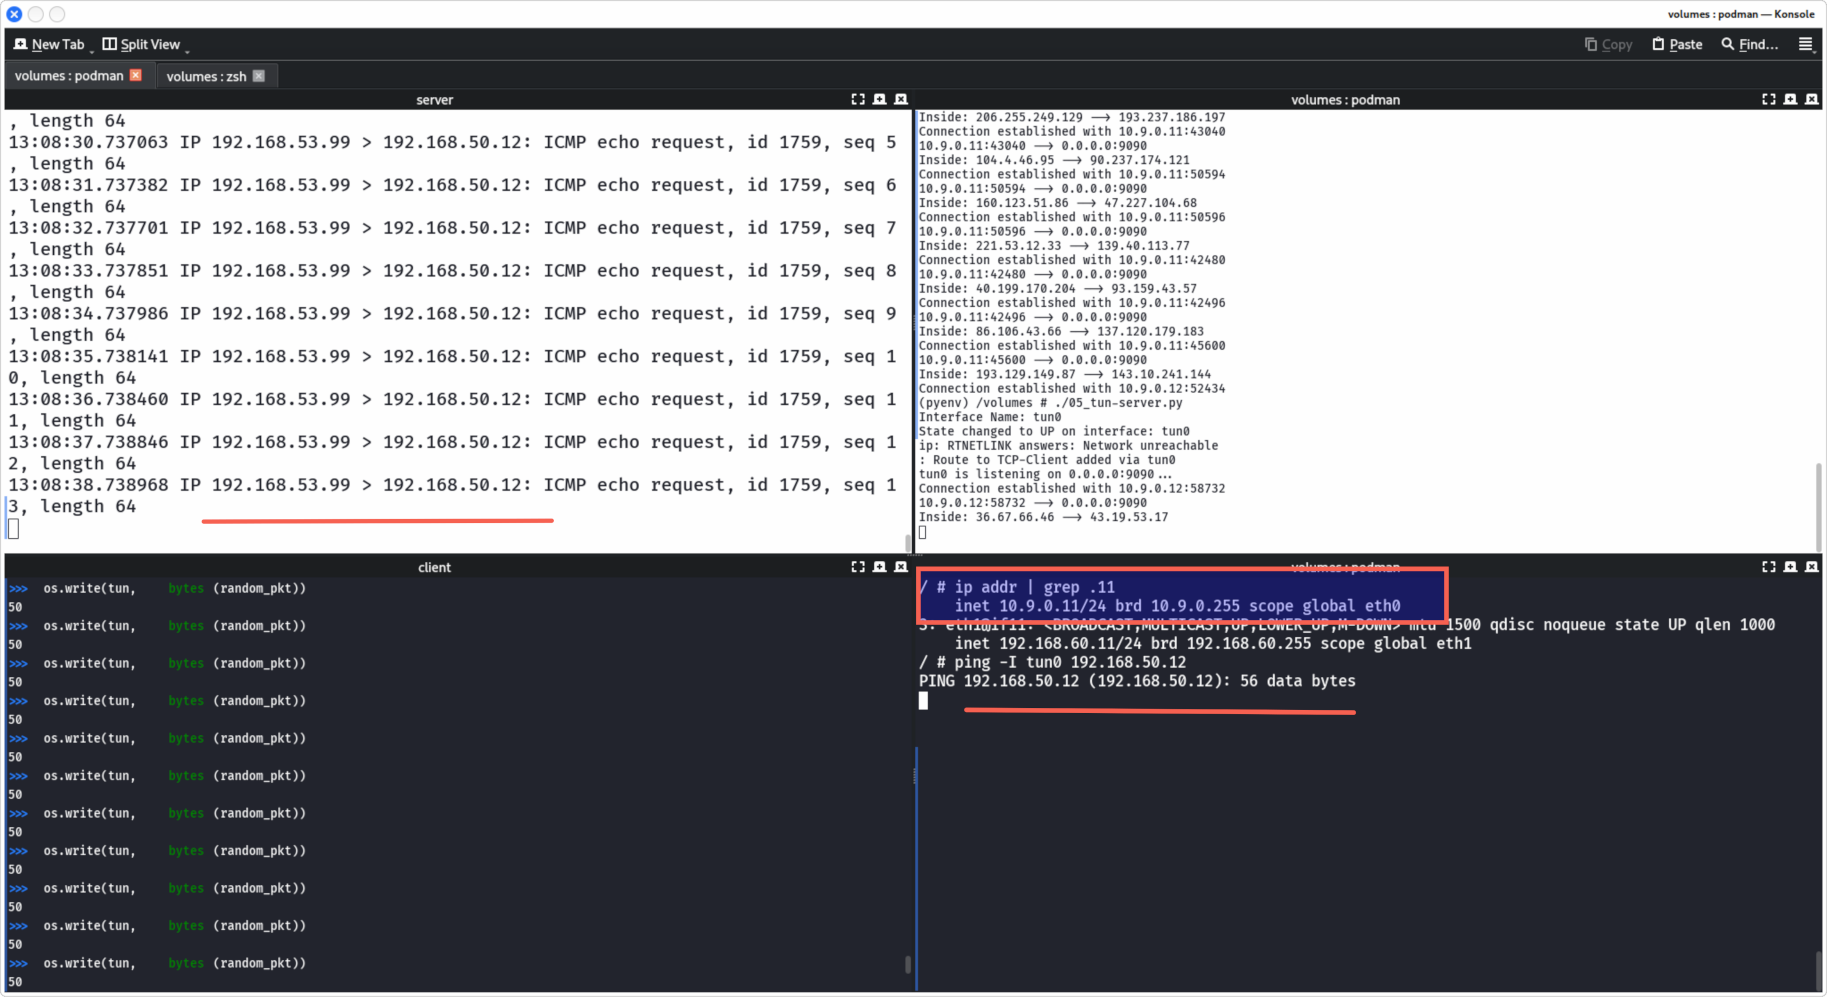
\includegraphics[width=0.5\linewidth]{Picture/03_lab-exercise-tunnel/06_bidirectional-ping-trough-tunnel.pdf.png}
    \caption{Bi-directional ping test trough interface \lstinline{tun0}}
    \label{fig:enter-label}
\end{figure}

\subsection{Building the TLS 1.2 Tunnel with Scapy}

At first step I tested the TLS connection on the same host targeting the loopback interface (with IPv4 Address: \lstinline{127.0.0.1}). 

For certification and key creation I generated a shell script, which calls the binary \lstinline{openssl} (\lstinline{/usr/bin/openssl}) with the appropriate parameters. For more detail on the parametrization of \lstinline{openssl} please refer to (Appendix \ref{\label{apx:sslkeygen} ).

The following codesnippets shows the client/server side code of reading and processing the generated keys/certification pairs (in PEM format):

\begin{lstlisting}[language=python, caption=Parse openssl keys and certification]
# Path to keyfiles and certifications
client_key = "ec_client.pem"  # Path to client's key: client.key (PEM-format)

# Read and load the PEM key
with open(client_key, "rb") as key_file:
    key_data = key_file.read()
    private_key = serialization.load_pem_private_key(key_data, password=None, backend=default_backend())

# Path certificate file (PEM format)
client_cert = "ec_client-cert.pem"

# Read and load the certificate
with open(client_cert, "rb") as cert_file:
    cert_data = cert_file.read()
    cert = x509.load_pem_x509_certificate(cert_data, default_backend())
\end{lstlisting}

Please note, I'm referring it as \textit{client/server} since I used the naming convention \lstinline{ec_[client|server].pem} for my output files generated by openssl (please refer to \textit{Appendix \ref{apx:sslkeygen}}).

To prepare the Server side for incoming connection I Instantiated the \lstinline{TLSServerAutomaton}  class as follows:

\begin{lstlisting}[language=python, caption=Create TLS Server with Scapy]
    
# Instantiate the TLSServerAutomaton class
tls_server = TLSServerAutomaton(
    server=IP_LISTEN, 
    sport=PORT_LISTEN, 
    mycert=server_cert,
    mykey=server_key,
    client_auth=True,           
    max_client_idle_time=50,    
    handle_session_ticket=None, 
    session_ticket_file=None,   # Session ticket file path
    curve="P-256"               # Choose curve parameter based on `tls.named_groups`
)

# Start the TLS server listening on: $IP_SERVER, $IPORT_LISTEN
tls_server.run()
\end{lstlisting}

( Please note I choosed the cipher suite for \textit{TLS1.3} from according \url{https://ciphersuite.info/cs/TLS_ECDHE_ECDSA_WITH_AES_128_GCM_SHA256/} as well as the curve parameter \lstinline{P-256}, but sadly I ran into several bugs, please refer to \textit{Appendix \ref{apx:ciphersuiteissues}}, so in my final implementation I commented out the parameter \lstinline{preferred_ciphersuite}.)

Similarly for the server side I modified the client's side code as the following:

\begin{lstlisting}[language=python, caption=Create TLS Client with Scapy]
# Testing Client Connection with/withouth ciphers: 
    client_automaton = TLSClientAutomaton.tlslink(
    server=SERVER_IP, 
    dport=SERVER_PORT,
    mycert=client_cert,
    mykey=client_key,
#    client_hello='TLS13ClientHello',
    proto="tls1_2"
    #version="tls13",
    # _tls.ciphersuites:
    #ciphers=["TLS_ECDHE_ECDSA_WITH_AES_128_GCM_SHA256"],
    #signature_algorithms=["ecdsa", "rsa"]  # Supported signature algorithms (adjust accordingly)
    )

\end{lstlisting}

In both Client/Server side's implementation the variables \lstinline{mycert,mykey} refers to the output files I generated with \lstinline{openssl} (Please refer to \ref{apx:sslkeygen}).

The following (\textit{Figure \ref{fig:tlshandshaketest}}) showcases the \lstinline{ClientHello} with a successfull TLS Handshake: 

\begin{figure}[h]
    \centering
    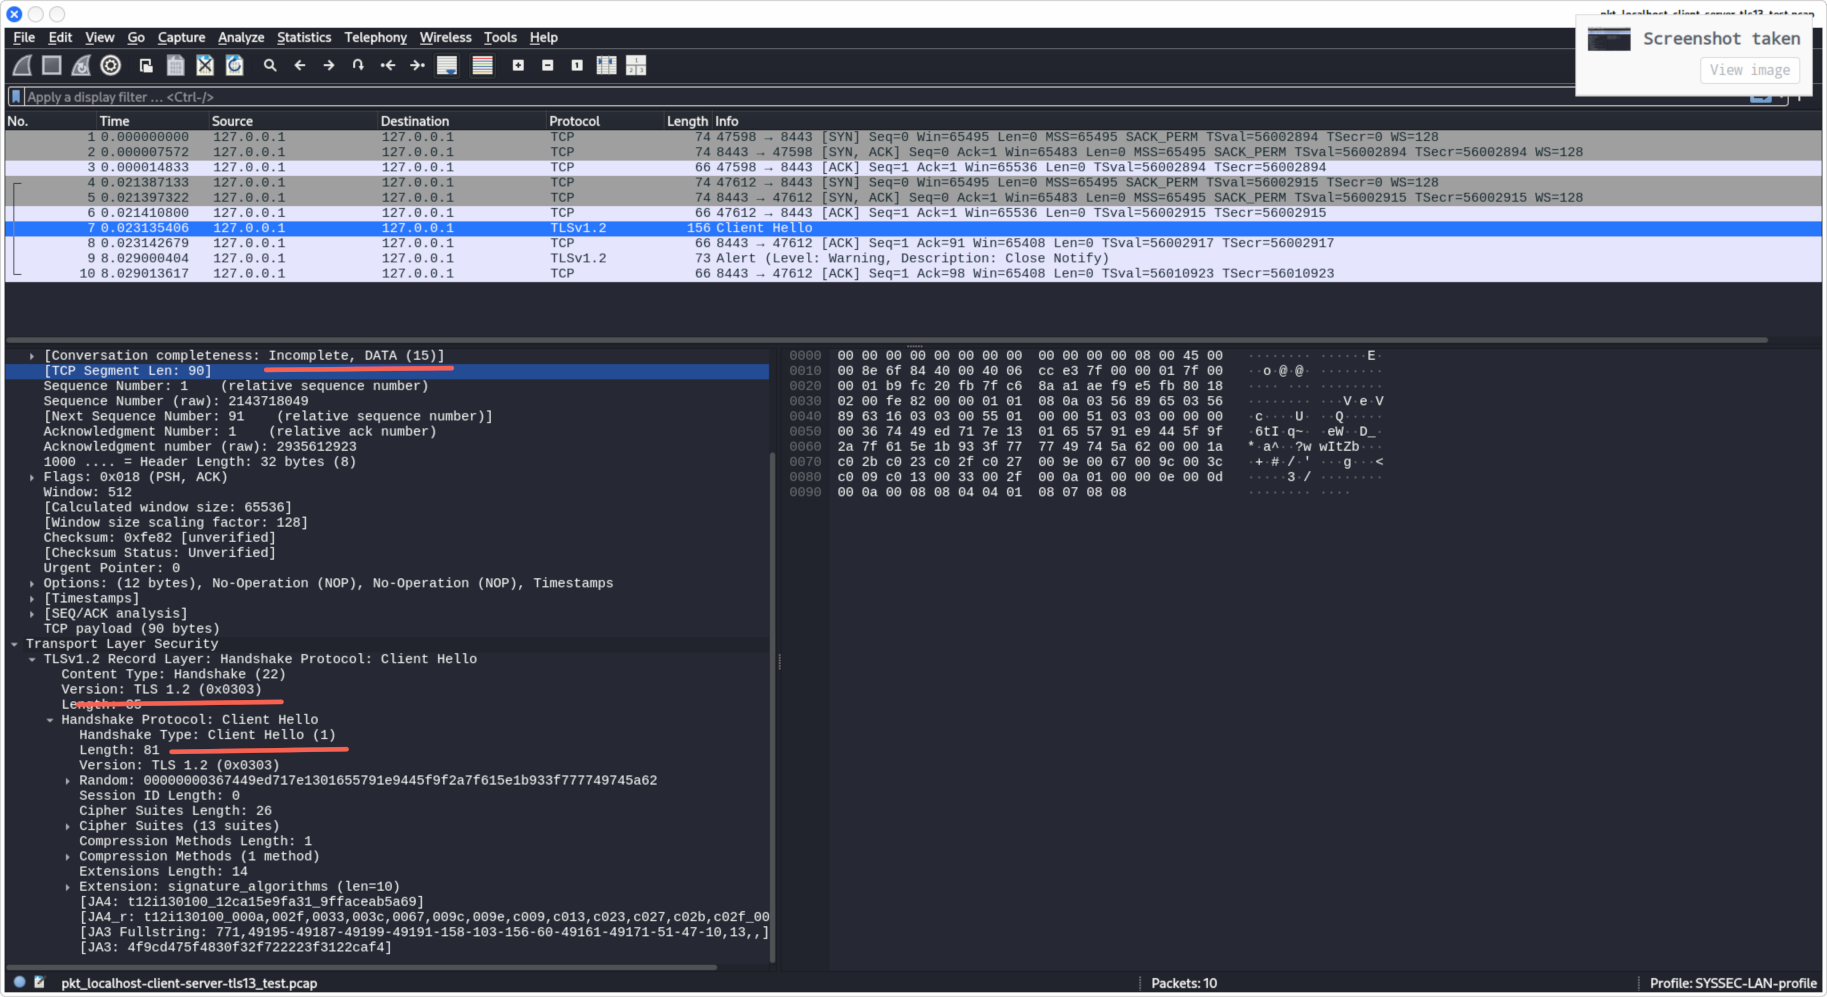
\includegraphics[width=0.5\linewidth]{Picture/03_lab-exercise-tunnel/100_tls_ClientHelloTest-start01.pdf.png}
    \caption{\lstinline{ClientHello} during TLS Handshake Test}
    \label{fig:tlshandshaketest}
\end{figure}

Last but not least for the actual implementation within \lstinline{13_client.py} the Server's \lstinline{IP} and \lstinline{PORT} address can be change back according to the network topology:

\begin{lstlisting}[language=python]
# Set TCP server according to network topology
SERVER_IP = "10.9.0.11"  # Server IP address
SERVER_PORT = 8443  # Server port, note please: for testing purpose I changed it to 9090
\end{lstlisting}

% 100_scapy-prompt-after-connection-established.pdf.png: 
\textit{Figure \ref{fig:clienttoserverconn}} showcases the \textit{Scapy} prompt for testing testing the client to server connection, after choosing parametrization \lstinline{proto="tls1_2"} for the connection.

\begin{figure}[h]
    \centering
    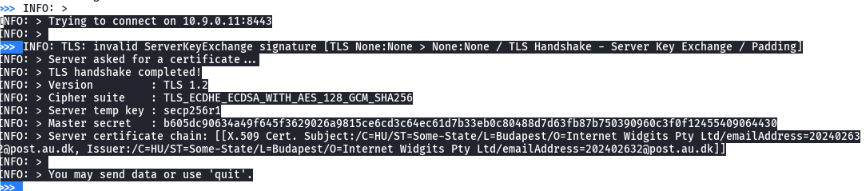
\includegraphics[width=0.9\linewidth]{Picture/03_lab-exercise-tunnel/100_scapy-prompt-after-connection-established.pdf.png}
    \caption{Testing \textit{Client} to \textit{Server} side connection with \lstinline{proto="tls1_2"}}
    \label{fig:clienttoserverconn}
\end{figure}

\subsection{Building the TLS 1.3 tunnel with ssl library}

To be able to set up the tls connection properly I rewrote this part as well as the scripts, ditching \lstinline{Scapy} completely (Please refer to \textit{Appendix: \ref{apx:scapy-issue}, \ref{apx:ciphersuiteissues}}) using \lstinline{ssl} library\cite{py.ssl}, with key generation as well according to \cite{tls.chain}.

(For the implementation please refer to the files \lstinline{00\_Rewrote-withouth-Scapy/01\_\_vpn-client-10.9.0.12/tls\_client.py}  and \lstinline{00_Rewrote-withouth-Scapy/01\_\_vpn-server-10.9.0.11/tls\_server.py}  )

% ref vissza a tunnel nelkuli bidirekciora
In \textit{Section } I showed the basic idea of sending and receiving bi-directional \textit{ICMP echo} requests and responses. The \textit{Figure} showcases the scenario after tunnel has been set up with the scripts \lstinline{tls_client.py} and \lstinline{tls_server.py}. The following snippet shows the \lstinline{tun0} interface routing setup according to  \lstinline{tls_server.py}. Please note that for the 

\textit{Client}'s side \lstinline{ 10.8.0.1/24 } address is changed to \lstinline{10.8.0.2/24} (Please refer to \lstinline{tls_client.py}).

\begin{lstlisting}[language=python, caption=Setting up \lstinline{tun0} interface on \lstinline{vpn-server}]
os.system(f"ip link set dev {ifname} up")
os.system(f"ip addr add 10.8.0.1/24 dev {ifname}")
os.system(f"ip route add 192.168.50.0/24 dev {ifname}")
\end{lstlisting}

After the tunnel is built up, I check the routing table for \lstinline{vpn-client} and \lstinline{vpn-server} as showcased in the following snippet. (Please note: This is the output of two consequent command )

\begin{lstlisting}[language=bash, caption=Checking the routing table on VPN-Client and VPN-Server after \lstinline{tun0} has been built up]
# Check Client route with: docker exec -it vpn-client-10.9.0.12 ip route
default via 192.168.50.1 dev eth1  metric 100 
10.8.0.0/24 dev tun0 scope link  src 10.8.0.2 
10.9.0.0/24 dev eth0 scope link  src 10.9.0.12 
192.168.50.0/24 dev eth1 scope link  src 192.168.50.12 
192.168.60.0/24 dev tun0 scope link 

# ...
# Check Server route with: docker exec -it vpn-server-10.9.0.11 ip route 
default via 192.168.60.1 dev eth1  metric 100 
10.8.0.0/24 dev tun0 scope link  src 10.8.0.1 
10.9.0.0/24 dev eth0 scope link  src 10.9.0.11 
192.168.50.0/24 dev tun0 scope link 
192.168.60.0/24 dev eth1 scope link  src 192.168.60.11 
\end{lstlisting}

For first I created the script \lstinline{00_keygen.sh} and \lstinline{cert.conf} key/certificate generation. Please refer to \textit{Appendix \ref{apx:openssl.keygenerator}} and the files mentioned to a comprehensive overview. For this assignment I used \lstinline{vpn-server-10.9.0.11} as the Certificate Authority\cite{tls.ca} (noted as \textit{CA} furthermore) and Intermediary Server\cite{tls.ca}, while referring \lstinline{vpn-client-10.9.0.12} as \textit{"User"}. (Please refer to \lstinline{00_keygen.sh} for more detailed view).

To be able to capture the \lstinline{TLS Handshake}\cite{tls} I listened on \lstinline{tun0} interface on the \textit{Server Side} while sending \lstinline{ICMP} packets explicitly (\lstinline{-I tun0} flag) trough the tunnel from \lstinline{vpn-client-10.9.0.12} to \lstinline{vpn-server-10.9.0.11} as can be seen on \textit{Figure \ref{fig:handshake-tls-client-to-server}}. For the complete handshake please refer to the file \lstinline{01_tls_tunnel_buildup__from-client-to-server.pcap}

%% TLS tunnel buildup: 
\begin{figure}[h]
    \centering
    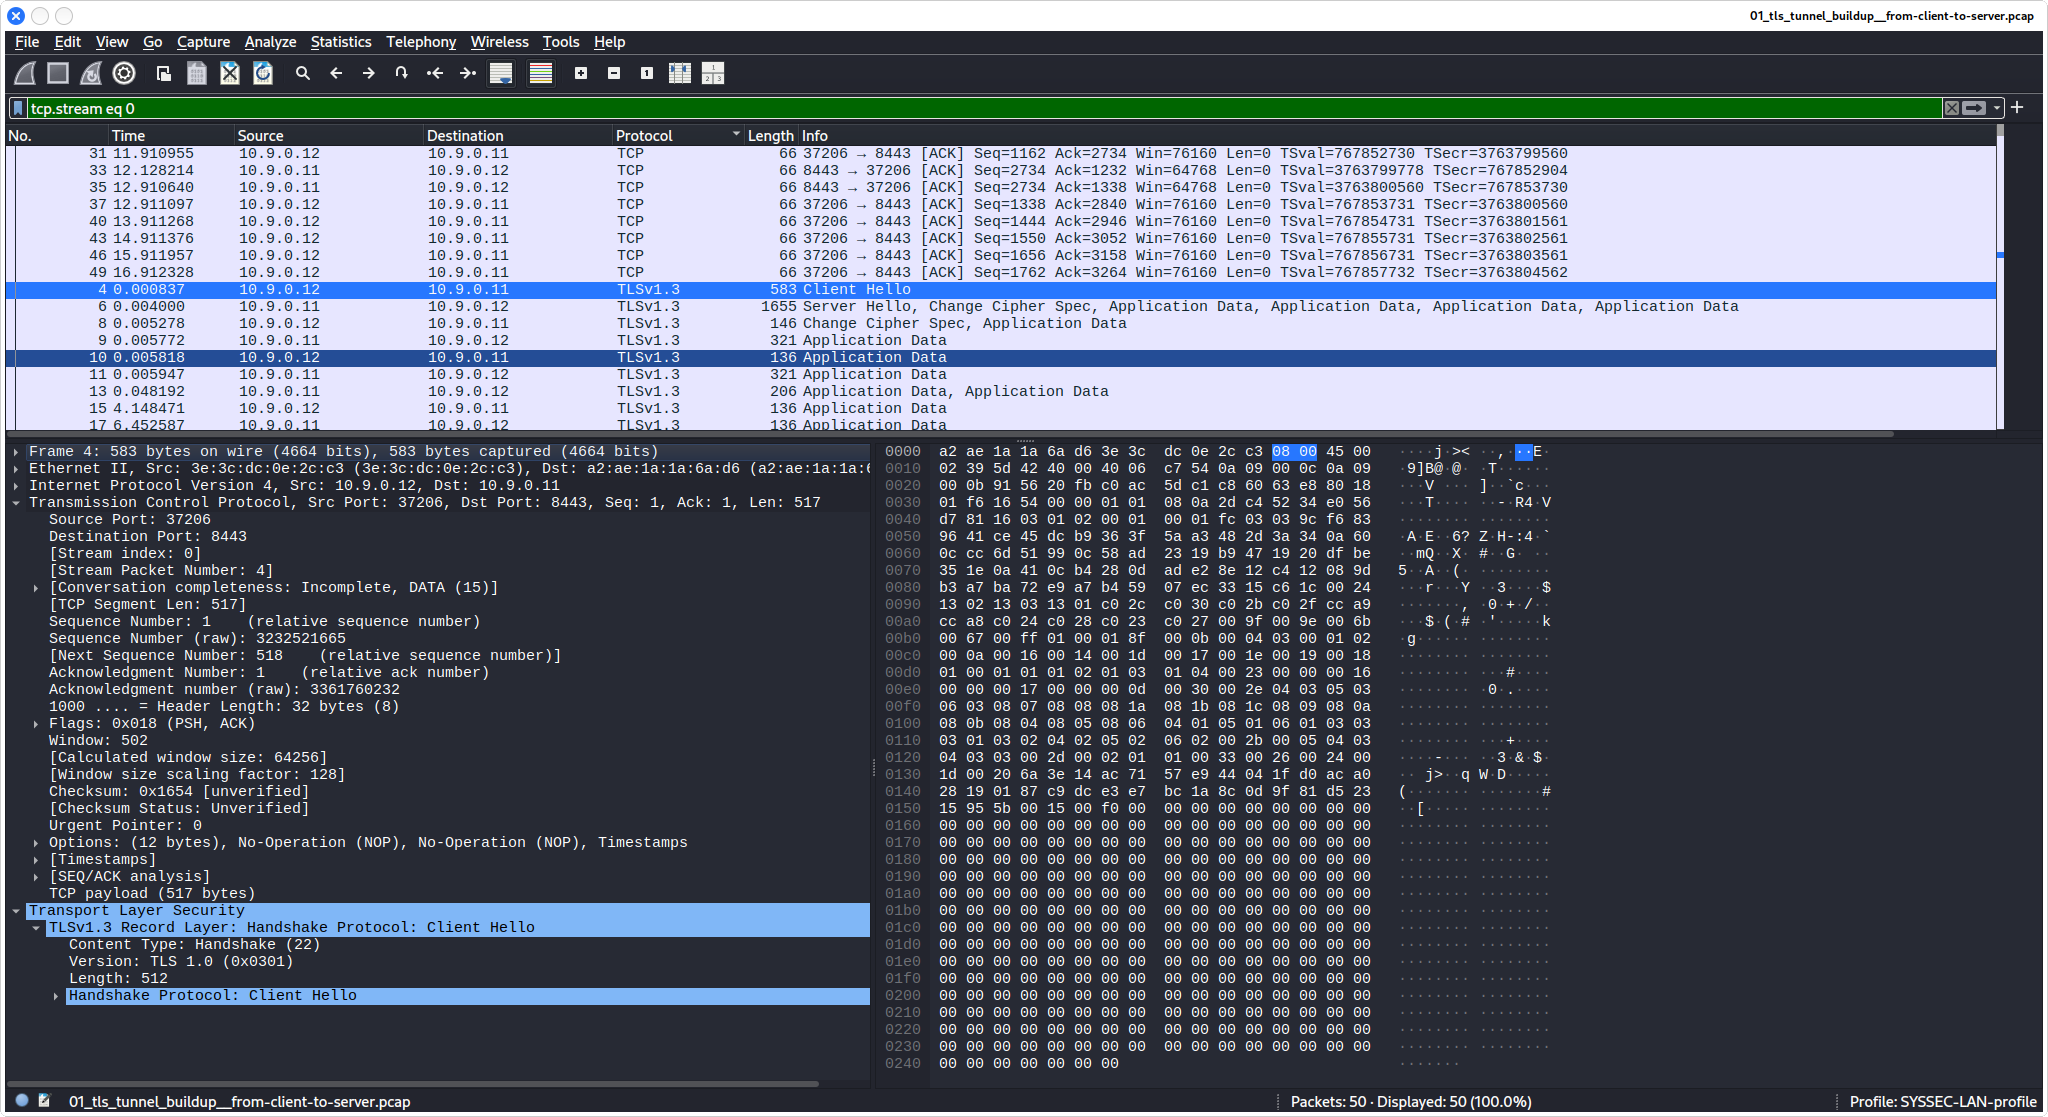
\includegraphics[width=0.5\linewidth]{Picture/04_final-with-ssl/routing-troubleshoot/01_tls_tunnel_buildup__from-client-to-server.pcap_001.png}
    \caption{Building TLS/SSL tunnel between \textit{VPN Client} and \textit{VPN Server} }
    \label{fig:handshake-tls-client-to-server}
\end{figure}

As can be seen on \textit{Figure \ref{fig:handshake-tls-client-to-server}} the connection is now using \lstinline{TLS 1.3} instead of \lstinline{TLS 1.2}\cite{tls13security} (Please refer to file: \lstinline{100_test-tls12-connection-scapy261-encrypted.pdf}). 

According to the network topology  as can be seen on \textit{Figure \ref{fig:networktopology}}, the \lstinline{TLS} handshake\cite{tlsssl.theory} will be initiated between the \textit{Client}'s and \textit{Server}'s \lstinline{eth0}interfaces configured for network \lstinline{10.9.0.0/24}. 

Now, the tunnel has been built up, I start a test to see that ICMP request gets the consequtive responses back from the tunnel as well as can be seen on \textit{Figure \ref{fig:vpn-tunnel-test-client-server}}: 

\begin{figure}[h]
    \centering
    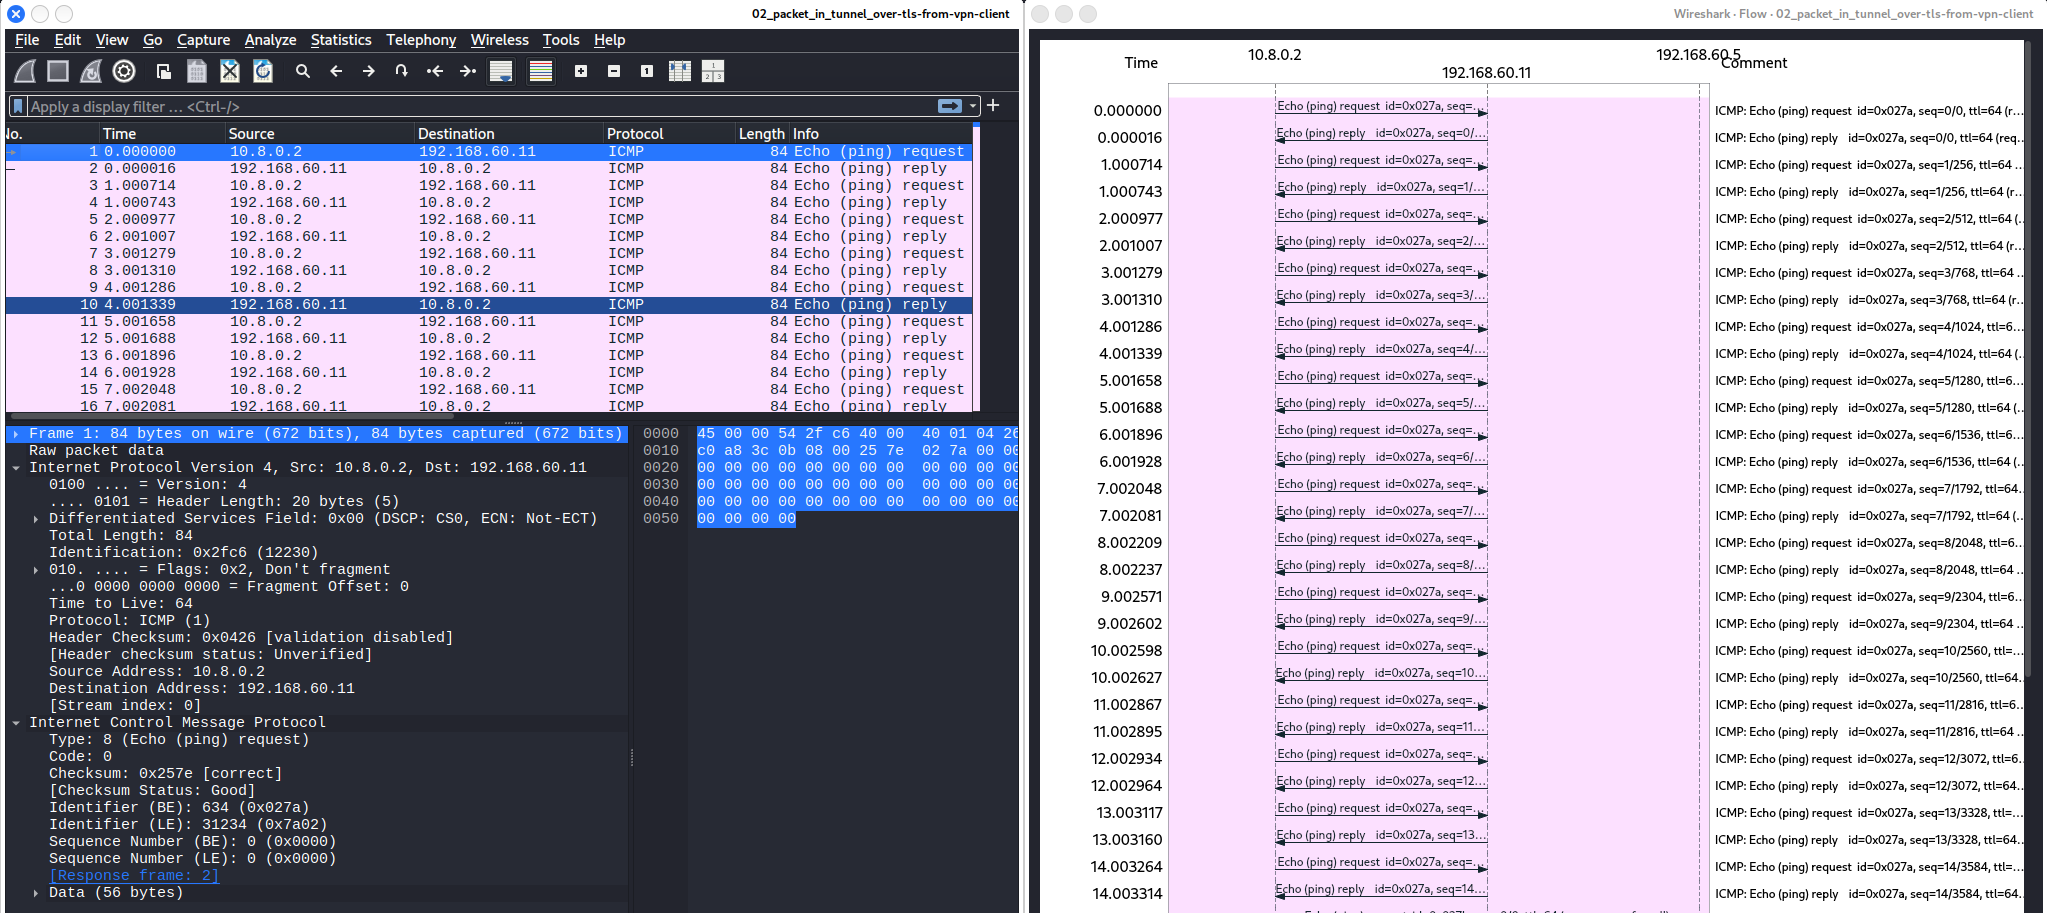
\includegraphics[width=0.5\linewidth]{Picture/04_final-with-ssl/routing-troubleshoot/02_packet_in_tunnel_over-tls-from-vpn-client-to-server.png}
    \caption{Sending and receiving ICMP echo requests and responses over the encrypted vpn tunnel}
    \label{fig:vpn-tunnel-test-client-server}
\end{figure}

A small note here, is that \lstinline{192.168.60.11} (which is the \lstinline{eth1} interface configured on \textit{VPN Server}) responds back to \lstinline{10.8.0.1} which is the \textit{Client}'s \lstinline{tun0} interface.     

\subsubsection{Bi-directional Connectivity test between \textit{Site A} and \textit{Site B}}
\label{sssec:bi-directional-ping}

As for now the tunnel has been successfully built up between \textit{Site A} (\lstinline{192.168.50.0/24}) and \textit{Site B}(\lstinline{192.168.60.0/24}), but I would like to reach the other hosts as well, not just the \textit{VPN Client/Server}. 

To to do so I want to make sure that \lstinline{IP} forwarding and routing has been set up properly on the \textit{VPN Client/Server}. Since I used \lstinline{sysctls}\cite{sysctl.conf} during the build time of containers (please refer to file \lstinline{VPN_LAB.yml}) I only need to test routing issues. 

\textit{Figure \ref{fig:routing-site-b}} shows the scenario for \textit{Site B} testing, with the command \lstinline{ping -I tun0 192.168.60.6} given out on \lstinline{vpn-client-10.9.0.12}. At first sight, it looks like \textit{ICMP} packets are being dropped completely, but that's not the case. 

\begin{figure}
    \centering
    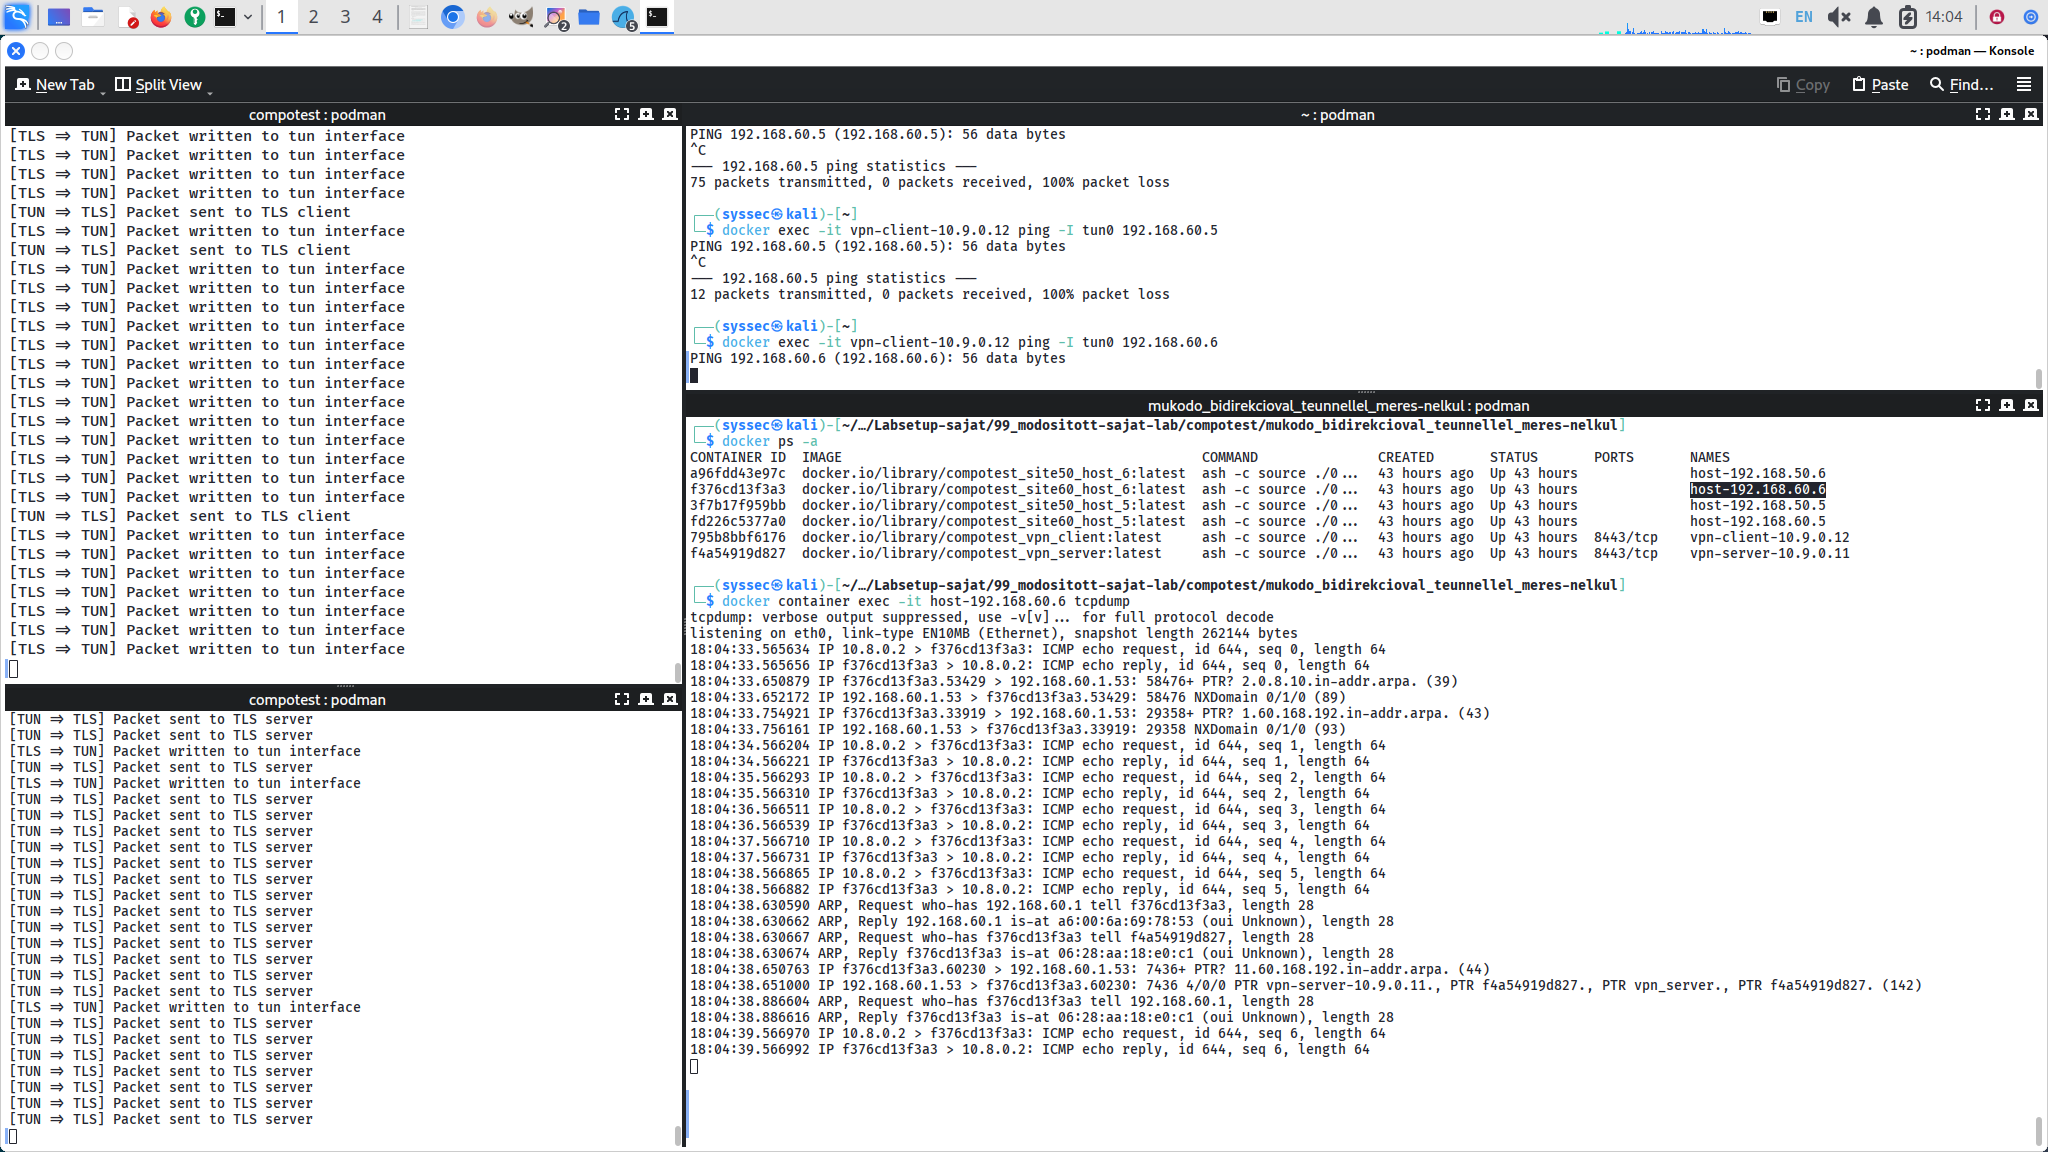
\includegraphics[width=0.5\linewidth]{Picture/04_final-with-ssl/routing-troubleshoot/04_pingtest_bidirection__vpn-client_to_192.168.60.6.png}
    \caption{Troubleshooting routing issues on \textit{Site B} hosts}
    \label{fig:routing-site-b}
\end{figure}

Listening on the \lstinline{eth0} interface of the target host \lstinline{192.168.60.6} clearly shows that the \textit{ICMP echo} requests are "hitting" \lstinline{192.168.60.6}, but for \lstinline{ICMP} response it sends back the packet to \lstinline{10.8.0.2}, which is the \textit{VPN Server}'s \lstinline{tun0} interface ( see \textit{Figure \ref{fig:networktopology}}). (For the similar tests against \textit{Site A} and \textit{Site B} hosts please see the images: 
    \lstinline{03_pingtest_bidirection__vpn-client_to_192.168.60.5.png}         
    \lstinline{04_pingtest_bidirection__vpn-client_to_192.168.60.6.png}          
    \lstinline{05_pingtest_bidirection__vpn-server_to_192.168.50.6.png}
    \lstinline{06_pingtest_bidirection__vpn-server_to_192.168.50.5.png}
)

% iptables on server/client to eth1/tun0 
To make sure that packets are not just forwarded but handled correctly between the  \lstinline{tun0} and \lstinline{eth1} interfaces  on hosts \textit{Client}, \textit{Server} I use the following \lstinline{iptables}\cite{bin.iptables} rules (please refer to the file \lstinline{routing_setup.sh}): 

\begin{lstlisting}[language=bash, caption=iptables rules to handle packets correctly]
# Server side
ip route add 192.168.60.0/24 dev eth1
iptables -A FORWARD -i eth1 -o tun0 -j ACCEPT
iptables -A FORWARD -i tun0 -o eth1 -j ACCEPT
iptables -t nat -A POSTROUTING -s 192.168.50.0/24 -o tun0 -j MASQUERADE

# Client side
ip route add 192.168.50.0/24 dev eth1
iptables -A FORWARD -i eth1 -o tun0 -j ACCEPT
iptables -A FORWARD -i tun0 -o eth1 -j ACCEPT
iptables -t nat -A POSTROUTING -s 192.168.60.0/24 -o tun0 -j MASQUERADE
\end{lstlisting}


Lastly I have to do is to correct the routing of \lstinline{192.168.60.6} regarding the network \lstinline{10.8.0.0/24}. The following code snippet shows the routing table of host \lstinline{192.168.60.6} before and after setting up the correct routing with command \lstinline{ip route add 10.8.0.0/24 via 192.168.60.11}. 

\begin{lstlisting}
# ip route BEFORE adding 10.8.0.0/24
default via 192.168.60.1 dev eth0  metric 100 
192.168.50.0/24 via 192.168.60.11 dev eth0 
192.168.60.0/24 dev eth0 scope link  src 192.168.60.6 

# ....
# ip route AFTER adding 10.8.0.0/24
default via 192.168.60.1 dev eth0  metric 100 
10.8.0.0/24 via 192.168.60.11 dev eth0 
192.168.50.0/24 via 192.168.60.11 dev eth0 
192.168.60.0/24 dev eth0 scope link  src 192.168.60.6 
\end{lstlisting}


\textit{Figure } shows the case for successfully initiated \textit{ICMP echo} response and request from \textit{VPN Client} to \lstinline{192.168.60.6} trough the vpn tunnel (according to Seed Lab Exercise):

\begin{figure}[h]
    \centering
    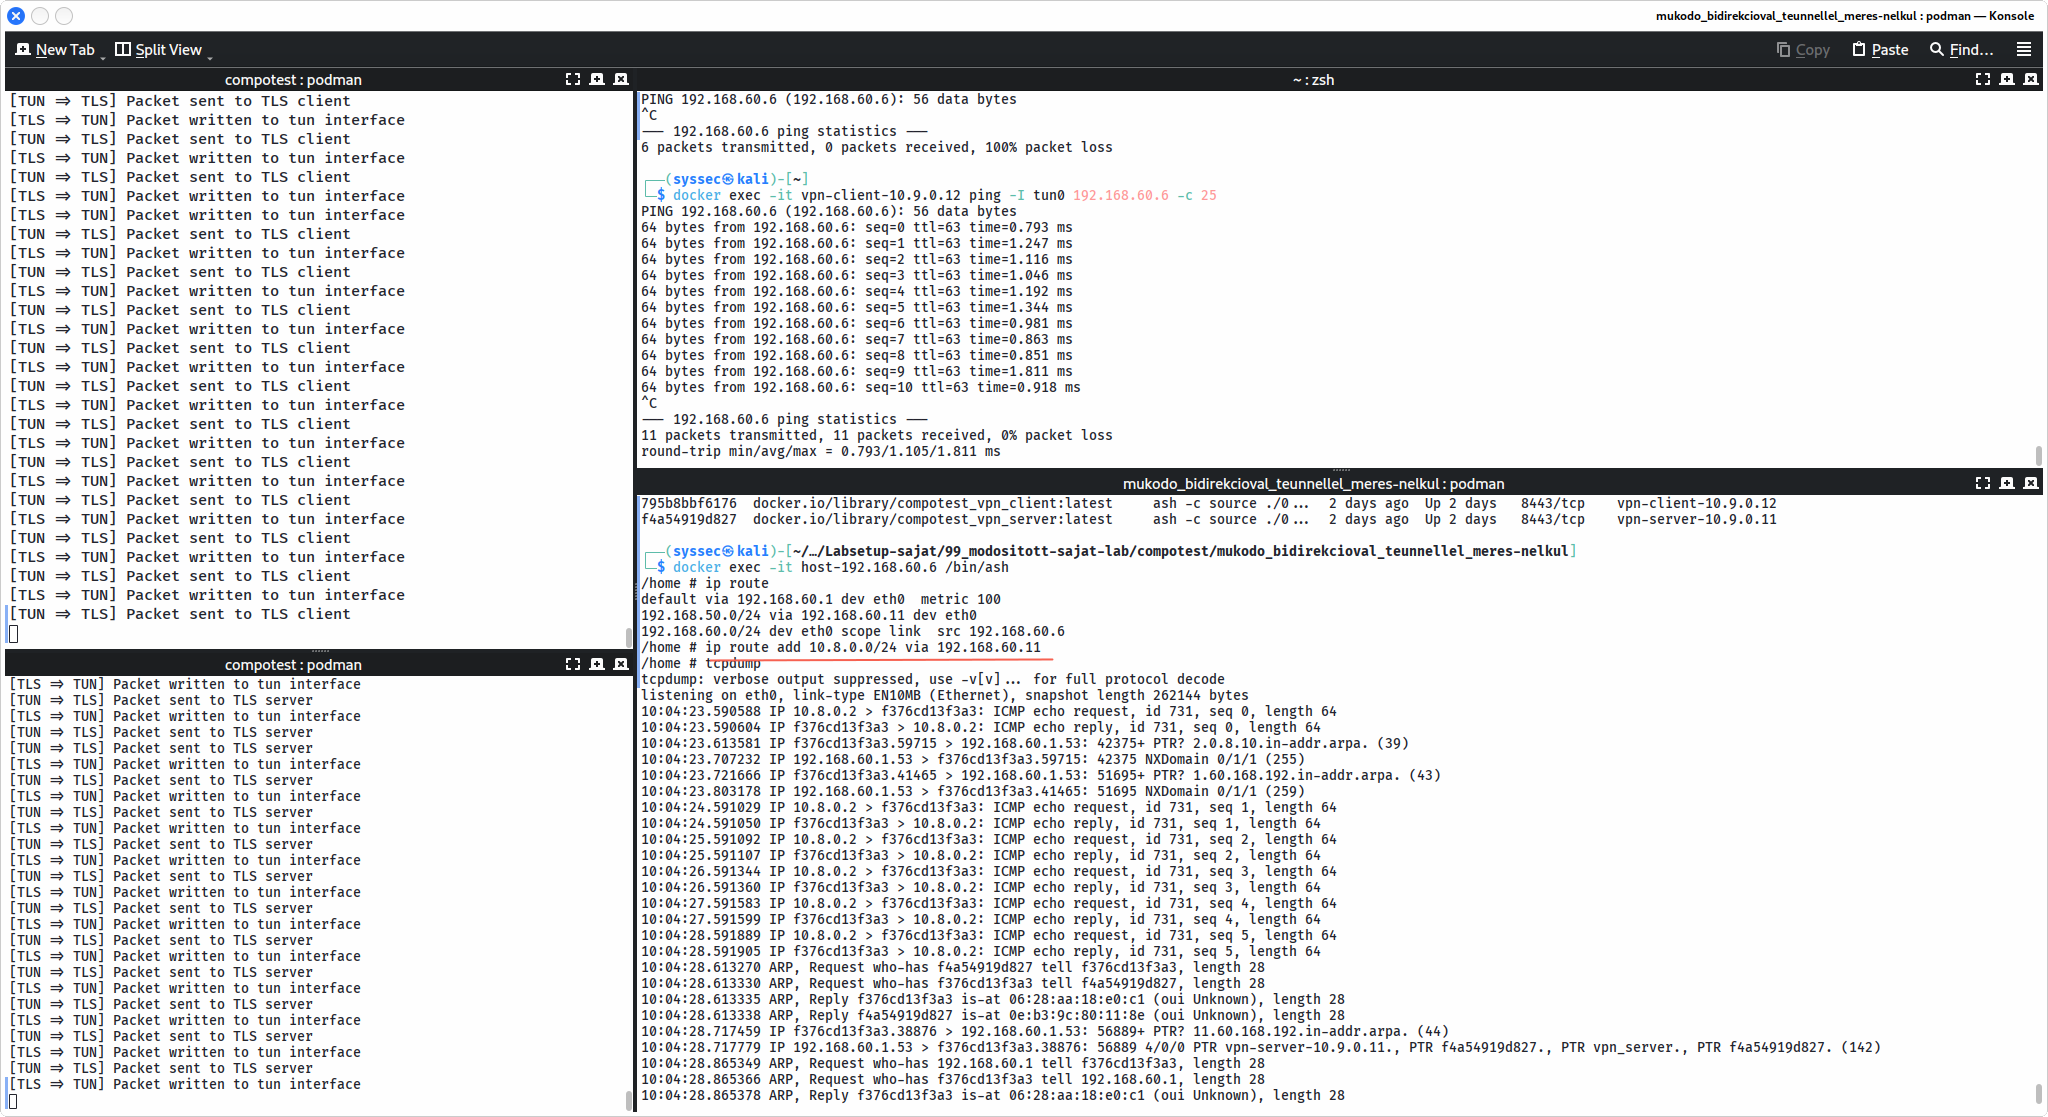
\includegraphics[width=0.5\linewidth]{Picture/04_final-with-ssl/04_pingtest_bidirection__vpn-client_to_192.168.60.6.routing.png}
    \caption{VPN tunnel Final Test}
    \label{fig:enter-label}
\end{figure}

The following code-snippet can be used to test the bi-directional IMCP echo requests and responses (please refer to \textit{Figure \ref{fig:pingfina;}}): 

\begin{lstlisting}[language=bash, caption=Testing the Site reachability from VPN Server and VPN Client]
echo "Ping Site B from VPN-Client"
echo "--------------------------------------------------------------------------"
docker exec -it vpn-client-10.9.0.12 ping -I tun0 192.168.60.11 -c -q 5
docker exec -it vpn-client-10.9.0.12 ping -I tun0 192.168.60.5  -c -q 5
docker exec -it vpn-client-10.9.0.12 ping -I tun0 192.168.60.6  -c -q 5
echo "--------------------------------------------------------------------------"

echo "Ping Site A from VPN-Server"
echo "--------------------------------------------------------------------------"
docker exec -it vpn-server-10.9.0.11 ping -I tun0 192.168.50.12 -c -q 5
docker exec -it vpn-server-10.9.0.11 ping -I tun0 192.168.50.5  -c -q 5
docker exec -it vpn-server-10.9.0.11 ping -I tun0 192.168.50.6  -c -q 5
echo "--------------------------------------------------------------------------"
\end{lstlisting}

\begin{figure}
    \centering
    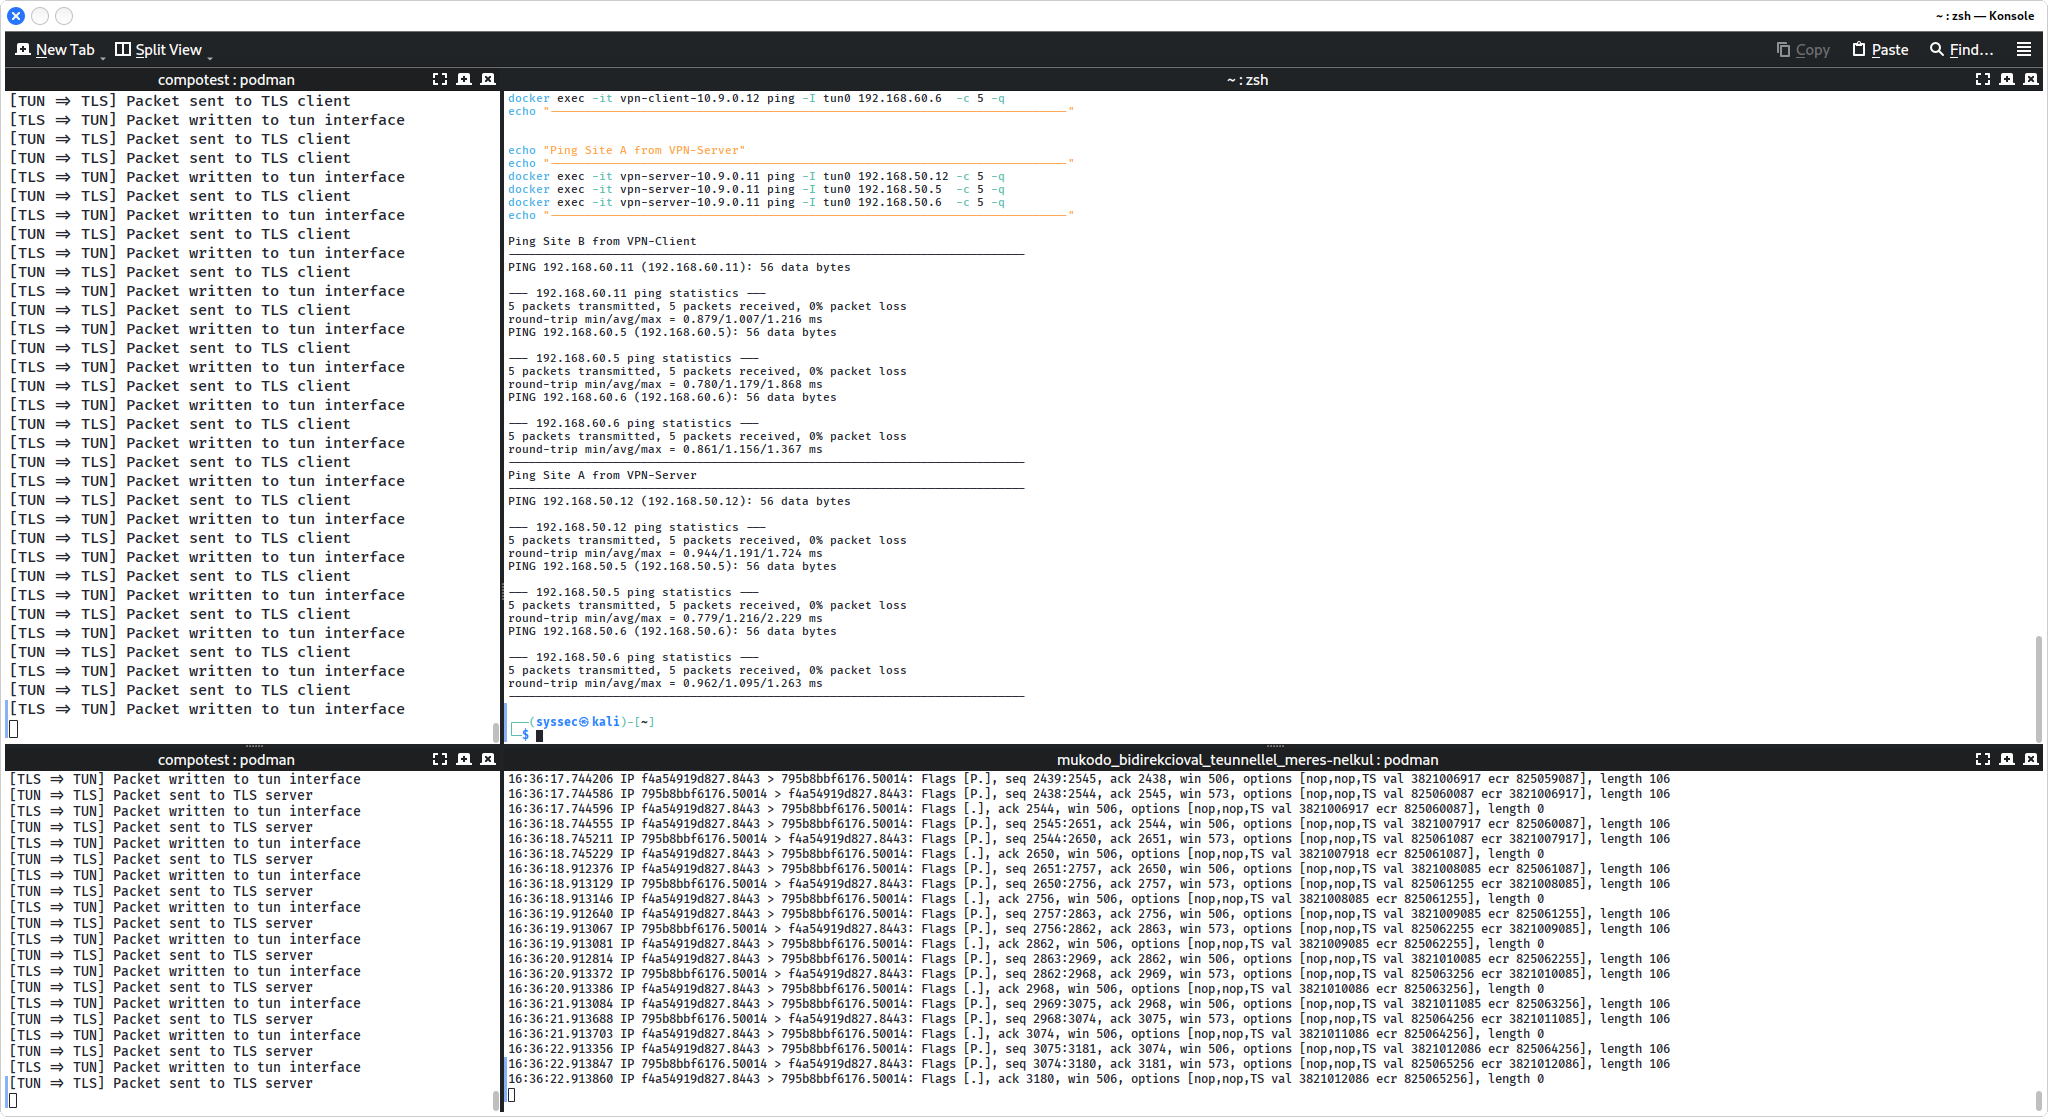
\includegraphics[width=0.5\linewidth]{Picture/04_final-with-ssl/07_pingtest.png}
    \caption{Testing site reachability from VPN Client and VPN Server}
    \label{fig:pingfina;}
\end{figure}


\newpage
\printbibliography
\newpage


% ========================================================
% Appendix
% ========================================================
\begin{appendix}
\section{Running the test without Building the Environment}
\input{Appendix/00_testrun}
\section{Host Environment Setup}
\section{Automated Building of Lab Environment on Kali Linux}
\label{apx:lab-final_envbuild}

For the second assignment for my Lab \textit{Host} system I choosed to use \textit{Kali Linux}\cite{os.kali}. 

The original documentation (please refer to: \cite{seedlab2024}) is referring to a pre-built \lstinline{*.iso} image denoted as \textit{Seed VM} which is based on the linux distribution Ubuntu (please refer to: \url{https://hub.docker.com/_/ubuntu}).  Since I'm not familiar with how they compiled the kernel nor which kernel modules are included or not in their custom Ubuntu container I built my own lab environment with slightly customization of the provided yml file \textit{docker-compose.yml} using Alpine Linux as a base for my container images.  For the container building process I used the tool called \textit{podman}\cite{podman}.

Podman is a daemonless, open source, Linux native tool designed to make it easy to find, run, build, share and deploy applications using Open Containers Initiative (OCI)\cite{oci.containers} Containers and Container Images.\cite{podman} Similarly to other common Container Engines (Docker, CRI-O, containerd), Podman relies on an OCI compliant Container Runtime (runc, crun, runv, etc) to interface with the operating system and create the running containers.\cite{podman} For the basic tasks we are able to simply make an alias to Docker to Podman (alias docker=podman) without any problems. 

\subsection{Cleanup the existing environment}

The \lstinline{VPN_LAB.yml} will build the whole lab environment from scratch, meaning that first the existing container images and networks should be removed:

\begin{lstlisting}[language=bash, caption=Host preparation for building the environment]
echo 'Delete previously created networks'
docker network rm --force "net-10.9.0.0"
docker network rm --force "net-192.168.50.0"
docker network rm --force "net-192.168.60.0"

echo 'Delete previously created containers'
docker stop host-192.168.50.5
docker stop host-192.168.50.6
docker stop host-192.168.60.5
docker stop host-192.168.60.6
docker stop host-vpn-server-10.9.0.11
docker stop host-client-server-10.9.0.12

docker rm host-192.168.50.5
docker rm host-192.168.50.6
docker rm host-192.168.60.5
docker rm host-192.168.60.6
docker rm host-vpn-server-10.9.0.11
docker rm host-client-server-10.9.0.12
\end{lstlisting}

Even tough in some cases if the container building process fails, some commit remains, this should be removed as well with \lstinline{docker image rm} command as can be seen of \textit{Figure \ref{fig:rmcon}}:

\begin{figure}[h]
    \centering
    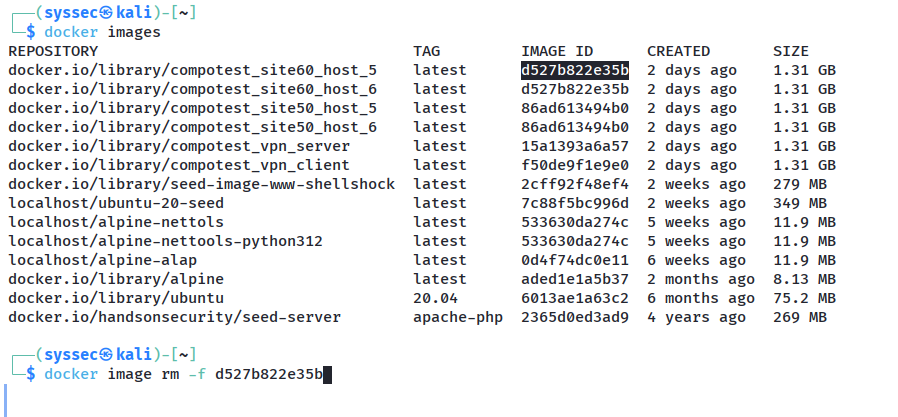
\includegraphics[width=0.5\linewidth]{Picture/00_Lab-Environment_Setup/999_docker-image-rm.png}
    \caption{Removing unnecessary container images}
    \label{fig:rmcon}
\end{figure}



\subsection{Review of \textit{Dockerfiles}\cite{docker.dockerfiles}}
\label{apx:lab-final_dockerfiles}

A \lstinline{Dockerfile} is basically a text document that contains all the necessary commands to call on the command line to assemble an image. For this specific lab I assembled four files according the network topology: \lstinline{Clientfile}, \lstinline{Serverfile}, \lstinline{SiteA}, \lstinline{SiteB} As an example I'll show snippets related to the container \lstinline{vpn-server-10.9.0.12}, but for a more comprehensive overview, please see the actual files I provided for the Assignment.

\subsubsection{Serverfile}
\label{apx:dockerfile.serverfile}

\begin{lstlisting}[language=bash,caption=Serverile overview for container vpn-server-10.9.0.11]
# ===========================================================
# Dockerfile for Building: VPN_SERVER
# ===========================================================

# Define container image
FROM alpine:latest

# Refresh repository
RUN apk update

# Install base packages
RUN apk add --no-cache busybox-extras tcpdump  texlive \
        tshark  graphviz  imagemagick  libpcap libpcap-dev \
        xdg-utils  openssl  openssl-dev   \
        graphviz imagemagick  sox  gcc  autoconf \
        curl vim nano python3 scapy iptables ca-certificates

# Install python3 and pip related packages
RUN apk add --no-cache python3 py3-matplotlib py3-cryptography python3-dev py3-pip

# Create python virtual environment
RUN python3 -m venv /opt/venv
COPY requirements.txt requirements.txt
RUN . /opt/venv/bin/activate && pip install -r requirements.txt

# Set server's listening port according to `tls_server.py`
EXPOSE 8443

WORKDIR /home/
COPY 00_keygen.sh /home/00_keygen.sh
COPY cert.conf /home/cert.conf
RUN chmod +x /home/00_keygen.sh
COPY tls_server.py /home/tls_server.py
RUN chmod +x /home/tls_server.py

# Add routing according to network topology
CMD ["/bin/ash", "ip route del default"]
CMD ["/bin/ash", "ip route add default via 10.9.0.1"]
CMD ["/bin/ash", "ip route add 192.168.60.0 via 192.168.60.11"]

# Build tunnel and tls client/server
#ENTRYPOINT ["python", "/home/tls_server.py", "--debug"]

\end{lstlisting}


\subsubsection{Clientfile}
\label{apx:dockerfile.clientfile}

The following code-snippet shows the \textit{Dockerfile} for automating the build process of \lstinline{vpn-client-10.9.0.12}

\begin{lstlisting}[language=bash, caption=Clientfile overview for container vpn-client-10.9.0.12]
# ===========================================================
# Dockerfile for Building: VPN_CLIENT
# ===========================================================

# Define container image
FROM alpine:latest

# Refresh repository
RUN apk update

# Install base packages
RUN apk add --no-cache busybox-extras tcpdump  texlive \
        tshark  graphviz  imagemagick  libpcap libpcap-dev \
        xdg-utils  openssl  openssl-dev   \
        graphviz imagemagick  sox  gcc  autoconf \
        curl vim nano python3 scapy iptables ca-certificates

# Install python3 and pip related packages
RUN apk add --no-cache python3 py3-matplotlib py3-cryptography python3-dev py3-pip

# Create python virtual environment
RUN python3 -m venv /opt/venv
COPY requirements.txt requirements.txt
RUN . /opt/venv/bin/activate && pip install -r requirements.txt

# Set server's listening port according to `tls_server.py`
EXPOSE 8443

WORKDIR /home/
COPY 00_keygen.sh /home/00_keygen.sh
COPY cert.conf /home/cert.conf
RUN chmod +x /home/00_keygen.sh
COPY tls_client.py /home/tls_client.py
RUN chmod +x /home/tls_client.py

# Add routing according to network topology
CMD ["/bin/ash", "ip route del default"]
CMD ["/bin/ash", "ip route add default via 10.9.0.1"]
CMD ["/bin/ash", "ip route add 192.168.50.0 via 192.168.50.12"]

# Build tunnel and tls client/server
#ENTRYPOINT ["python", "/home/tls_client.py", "--debug"]

\end{lstlisting}

\subsubsection{SiteA}

\begin{lstlisting}[language=bash, caption=Overview of SiteA dockerfile for containers within the subnet 192.168.50.0/24]
# ===========================================================
# Dockerfile for Building: SITE_A (192.168.50.0/24)
# ===========================================================

# Define container image
FROM alpine:latest

# Refresh repository
RUN apk update

# Install base packages
RUN apk add --no-cache busybox-extras tcpdump  texlive \
        tshark  graphviz  imagemagick  libpcap libpcap-dev \
        xdg-utils  openssl  openssl-dev   \
        graphviz imagemagick  sox  gcc  autoconf \
        curl vim nano python3 scapy iptables ca-certificates

# Install python3 and pip related packages
RUN apk add --no-cache python3 py3-matplotlib py3-cryptography python3-dev py3-pip

# Create python virtual environment
RUN python3 -m venv /opt/venv
COPY requirements.txt requirements.txt
RUN . /opt/venv/bin/activate && pip install -r requirements.txt

# Add routing according to network topology
CMD ["/bin/ash", "ip route del default"]
CMD ["/bin/ash", "ip route add default via 192.168.50.12"]
CMD ["/bin/ash", "ip route add 192.168.60.0/24 via 192.168.50.12"]

# Generate keys/certificates
WORKDIR /home/
COPY 00_keygen.sh /home/00_keygen.sh
COPY cert.conf /home/cert.conf
RUN chmod +x /home/00_keygen.sh

\end{lstlisting}

\subsubsection{SiteB}
\begin{lstlisting}[language=bash, caption=Overview of SiteB dockerfile for containers within subnet 192.168.60.0/24]
# ===========================================================
# Dockerfile for Building: SITE_B (192.168.60.0/24)
# ===========================================================

# Define container image
FROM alpine:latest

# Refresh repository
RUN apk update

# Install base packages
RUN apk add --no-cache busybox-extras tcpdump  texlive \
        tshark  graphviz  imagemagick  libpcap libpcap-dev \
        xdg-utils  openssl  openssl-dev   \
        graphviz imagemagick  sox  gcc  autoconf \
        curl vim nano python3 scapy iptables ca-certificates

# Install python3 and pip related packages
RUN apk add --no-cache python3 py3-matplotlib py3-cryptography python3-dev py3-pip

# Create python virtual environment
RUN python3 -m venv /opt/venv
COPY requirements.txt requirements.txt
RUN . /opt/venv/bin/activate && pip install -r requirements.txt

# Add routing according to network topology
CMD ["/bin/ash", "ip route del default"]
CMD ["/bin/ash", "ip route add default via 192.168.60.11"]
CMD ["/bin/ash", "ip route add 192.168.50.0/24 via 192.168.60.11"]

# Generate keys/certificates
WORKDIR /home/
COPY 00_keygen.sh /home/00_keygen.sh
COPY ca.conf /home/ca.conf
RUN chmod +x /home/00_keygen.sh

\end{lstlisting}

\subsubsection{Overview of requirements.txt}

\begin{lstlisting}[language=python, caption=Overview of requirements.txt]
    alabaster==1.0.0
astroid==3.3.9
asttokens==3.0.0
babel==2.17.0
certifi==2025.1.31
cffi==1.17.1
charset-normalizer==3.4.1
contourpy==1.3.1
cryptography==44.0.2
cycler==0.12.1
decorator==5.2.1
dill==0.3.9
docutils==0.21.2
executing==2.2.0
fonttools==4.56.0
graphviz==0.20.3
idna==3.10
imagesize==1.4.1
ipython==9.0.2
ipython_pygments_lexers==1.1.1
isort==6.0.1
jedi==0.19.2
Jinja2==3.1.6
kiwisolver==1.4.8
MarkupSafe==3.0.2
matplotlib==3.10.1
matplotlib-inline==0.1.7
mccabe==0.7.0
numpy==2.2.3
p0f==1.0.0
packaging==24.2
parso==0.8.4
pexpect==4.9.0
pillow==11.1.0
platformdirs==4.3.7
prompt_toolkit==3.0.50
ptyprocess==0.7.0
pure_eval==0.2.3
pycparser==2.22
pycryptodome==3.22.0
Pygments==2.19.1
pylint==3.3.6
pyparsing==3.2.1
python-dateutil==2.9.0.post0
PyX==0.16
pyxi==0.1.4
requests==2.32.3
roman-numerals-py==3.1.0
setuptools==78.1.0
six==1.17.0
snowballstemmer==2.2.0
Sphinx==8.2.3
sphinx-rtd-theme==3.0.2
sphinxcontrib-applehelp==2.0.0
sphinxcontrib-devhelp==2.0.0
sphinxcontrib-htmlhelp==2.1.0
sphinxcontrib-jquery==4.1
sphinxcontrib-jsmath==1.0.1
sphinxcontrib-qthelp==2.0.0
sphinxcontrib-serializinghtml==2.0.0
stack-data==0.6.3
tinyec==0.4.0
tomlkit==0.13.2
traitlets==5.14.3
urllib3==2.3.0
wcwidth==0.2.13
wheel

\end{lstlisting}


\subsection{Review of \textit{VPN\_LAB.yml} file}
The container environment can be built automatically with the following \lstinline{.yml} file, with command: \lstinline{podman compose --file VPN_LAB.yml up --force-recreate --detach}


\begin{lstlisting}[language=bash, caption=Building lab environment based on VPN\_LAB.yml]
version: "3"

services:
    vpn_client:
        build:
            context: .
            dockerfile: Clientfile
        container_name: vpn-client-10.9.0.12
        tty: true
        cap_add:
                - ALL
        devices:
                - "/dev/net/tun:/dev/net/tun"
        sysctls:
                - net.ipv4.ip_forward=1
        volumes:
                - ./volumes:/volumes
        networks:
            net-10.9.0.0:
                ipv4_address: 10.9.0.12
            net-192.168.50.0:
                ipv4_address: 192.168.50.12
        command: ash -c "source ./00_keygen.sh && host_keygen client && host_keygen server && inetd start && tail -f /dev/null"

    vpn_server:
        build:
            context: .
            dockerfile: Serverfile
        container_name: vpn-server-10.9.0.11
        tty: true
        cap_add:
                - ALL
        devices:
                - "/dev/net/tun:/dev/net/tun"
        sysctls:
                - net.ipv4.ip_forward=1
        volumes:
                - ./volumes:/volumes
        networks:
            net-10.9.0.0:
                ipv4_address: 10.9.0.11
            net-192.168.60.0:
                ipv4_address: 192.168.60.11
        command: ash -c "source ./00_keygen.sh && host_keygen client && host_keygen server && inetd start && tail -f /dev/null"

    site50_host_5:
        build:
            context: .
            dockerfile: SiteA
        container_name: host-192.168.50.5
        tty: true
        cap_add:
                - ALL
        networks:
            net-192.168.50.0:
                ipv4_address: 192.168.50.5
        command: ash -c "source ./00_keygen.sh && host_keygen client && inetd start && tail -f /dev/null"

    site50_host_6:
        build:
            context: .
            dockerfile: SiteA
        container_name: host-192.168.50.6
        tty: true
        cap_add:
                - ALL
        networks:
            net-192.168.50.0:
                ipv4_address: 192.168.50.6
        command: ash -c "source ./00_keygen.sh  && host_keygen client && inetd start && tail -f /dev/null"

    site60_host_5:
        build:
            context: .
            dockerfile: SiteB
        container_name: host-192.168.60.5
        tty: true
        cap_add:
                - ALL
        networks:
            net-192.168.60.0:
                ipv4_address: 192.168.60.5
        command: ash -c "source ./00_keygen.sh  && host_keygen client && inetd start && tail -f /dev/null"

    site60_host_6:
        build:
            context: .
            dockerfile: SiteB
        container_name: host-192.168.60.6
        tty: true
        cap_add:
                - ALL
        networks:
            net-192.168.60.0:
                ipv4_address: 192.168.60.6
        command: ash -c "source ./00_keygen.sh  && host_keygen client && inetd start && tail -f /dev/null"

networks:
    net-192.168.50.0:
        name: net-192.168.50.0
        ipam:
            config:
                - subnet: 192.168.50.0/24
    net-192.168.60.0:
        name: net-192.168.60.0
        ipam:
            config:
                - subnet: 192.168.60.0/24

    net-10.9.0.0:
        name: net-10.9.0.0
        ipam:
            config:
                - subnet: 10.9.0.0/24


\end{lstlisting}

% Kiegeszito file-ok + lista, hogy melyik file mit takar
\section{Auxiliary files}
\input{Appendix/99_UP202504__aux-file-list}


\section{Packet Structures and \textit{Scapy Layers} }
\subsection{Scapy Ethernet Layer}
\label{apx:ethernet}

One can use the command \lstinline{ls(Ether)} to get an information about \textit{Scapy}'s \cite{scapy2024} \lstinline{Ethernet} layer:

\begin{lstlisting}[language=python, caption=Scapy Ether Layer]
dst        : DestMACField                        = ('None')
src        : SourceMACField                      = ('None')
type       : XShortEnumField                     = ('36864')
\end{lstlisting}

One can use the command \lstinline{ls(ARP)} to get an information about \textit{Scapy}'s \cite{scapy2024} \lstinline{ARP} layer:

\begin{lstlisting}[language=python, caption=Scapy ARP Layer]
hwtype     : XShortEnumField                     = ('1')
ptype      : XShortEnumField                     = ('2048')
hwlen      : FieldLenField                       = ('None')
plen       : FieldLenField                       = ('None')
op         : ShortEnumField                      = ('1')
hwsrc      : MultipleTypeField (SourceMACField, StrFixedLenField) = ('None')
psrc       : MultipleTypeField (SourceIPField, SourceIP6Field, StrFixedLenField) = ('None')
hwdst      : MultipleTypeField (MACField, StrFixedLenField) = ('None')
pdst       : MultipleTypeField (IPField, IP6Field, StrFixedLenField) = ('None')
\end{lstlisting}

\subsection{Scapy IP version 4 Layer}
\label{apx:ipv4}

One can use the command \lstinline{ls(IP)} to get an information about \textit{Scapy}'s \cite{scapy2024} \lstinline{IP} layer:

\begin{lstlisting}[language=python, caption=Scapy IPv4 Layer]
version    : BitField  (4 bits)                  = ('4')
ihl        : BitField  (4 bits)                  = ('None')
tos        : XByteField                          = ('0')
len        : ShortField                          = ('None')
id         : ShortField                          = ('1')
flags      : FlagsField                          = ('<Flag 0 ()>')
frag       : BitField  (13 bits)                 = ('0')
ttl        : ByteField                           = ('64')
proto      : ByteEnumField                       = ('0')
chksum     : XShortField                         = ('None')
src        : SourceIPField                       = ('None')
dst        : DestIPField                         = ('None')
options    : PacketListField                     = ('[]')
\end{lstlisting}
\subsection{Scapy ICMP Layer}
\label{apx:icmp}

One can use the command \lstinline{ls(ICMP)} to get an information about \textit{Scapy}'s \cite{scapy2024} \lstinline{ICMP} layer:

\begin{lstlisting}[language=python, caption=Scapy ICMP Layer]
type       : ByteEnumField                       = ('8')
code       : MultiEnumField (Depends on 8)       = ('0')
chksum     : XShortField                         = ('None')
id         : XShortField (Cond)                  = ('0')
seq        : XShortField (Cond)                  = ('0')
ts_ori     : ICMPTimeStampField (Cond)           = ('72829031')
ts_rx      : ICMPTimeStampField (Cond)           = ('72829031')
ts_tx      : ICMPTimeStampField (Cond)           = ('72829031')
gw         : IPField (Cond)                      = ("'0.0.0.0'")
ptr        : ByteField (Cond)                    = ('0')
reserved   : ByteField (Cond)                    = ('0')
length     : ByteField (Cond)                    = ('0')
addr_mask  : IPField (Cond)                      = ("'0.0.0.0'")
nexthopmtu : ShortField (Cond)                   = ('0')
unused     : MultipleTypeField (ShortField, IntField, StrFixedLenField) = ("b''")
extpad     : _ICMPExtensionPadField (Cond)       = ("b''")
ext        : _ICMPExtensionField (Cond)          = ('None')
\end{lstlisting}

Where \lstinline{type} refers to \lstinline{ICMP} type according to \lstinline{RFC 792}, \lstinline{RFC 2780}
\subsection{TCP Packet Structure}
\label{apx:tcp}

One can use the command \lstinline{ls(TCP)} to get an information about \textit{Scapy}'s \cite{scapy2024} \lstinline{TCP} layer:

\begin{lstlisting}[language=python, caption=Scapy TCP Layer]
version    : BitField  (4 bits)                  = ('4')
ihl        : BitField  (4 bits)                  = ('None')
tos        : XByteField                          = ('0')
len        : ShortField                          = ('None')
id         : ShortField                          = ('1')
flags      : FlagsField                          = ('<Flag 0 ()>')
frag       : BitField  (13 bits)                 = ('0')
ttl        : ByteField                           = ('64')
proto      : ByteEnumField                       = ('0')
chksum     : XShortField                         = ('None')
src        : SourceIPField                       = ('None')
dst        : DestIPField                         = ('None')
options    : PacketListField                     = ('[]')
\end{lstlisting}


    
\section{Key generation for \textit{Client} and \textit{Server} with \lstinline{openssl}}
For Client and Server key/certificate generation I used the program \lstinline{openssl}\ref{openssl.keygen}.

The following code snippet showcases the \textit{Server} key generation of \lstinline{00_keygen.sh} script. Please note: For the actual test environment, the \lstinline{00_keygen.sh} should be sourced\cite{shell.bash} within the container environment,as can be seen within the \textit{Dockerfiles}\ref{apx:dockerfile.serverfile, apx:dockerfile.clientfile}

\subsection{Overview of openssl key generation with \textit{00\_keygen.sh}}
\label{apx:lab-final_keygen}

\begin{lstlisting}[language=bash, caption=openssl keygeneration script]
#!/bin/ash

# ========================================
# Openssl key/certificate generator script
# ----------------------------------------

# Host Key/Certification generation according to `cert.conf` contents.
# The functions accepts 2 input parameters:
# 	`server`	:= server key/certificate generation
# 	`client` 	:= client key/certificate generation 

# Please note: For this assignment I vpn-server is the same as CA and Intermediary Server

# The file is being sourced trough dotfiles, hence
# the function is usable as a command as follows:
#
# host_keygen server	:= generates server ca/key
# host_keygen client	:= generates client ca/key

# Please note: The script is meant to be used as beign sourced
# Please refer to the `source` command arguments in the dockerfiles
host_keygen() {

echo
echo "======================================================"
echo "Client/Server keypair generation using OpenSSL library"
echo "======================================================"
echo

# Choose Server/Client
HOST_MODE=$1
	case $HOST_MODE in
		
		# Generating server key/certificate using group 'prime256v1' according to RFC 3279
		server)
	
		export NAME_TAG="$(hostname)"
		export CERT_CONF="cert.conf"
		export CA_KEY_NAME="CA_KeyFile"
		export CA_CERT_NAME="CA_Certificate"
		export TRUST_STORE="/etc/ssl/certs/"
		export TRUST_KEY_STORE="/etc/ssl/private/"
		export SHARED_DIR="/volumes/inter"
			echo
			echo "Generating the Root CA certificate as $NAME_TAG"
			echo "---------------------------------------------------------"
			echo
			
				# Key/CA generation based on 2048-bit RSA
				# .......................................
				openssl genrsa -out "$CA_KEY_NAME".pem 2048
				
				echo "Generate the Root CA's self-signed certificate: "
				echo "---------------------------------------------------------"
				openssl req -new -x509 -days 365 -sha256 -key "$CA_KEY_NAME".pem -config "$CERT_CONF" -out "$CA_CERT_NAME".crt

				echo 'Check Certificate Content:'
				echo "---------------------------------------------------------"
				openssl x509 -in "$CA_CERT_NAME".crt -text -noout

				# Key/CA generation based on Elliptice Curves
				# ...........................................
				# Store keyfiles un-encrypted on disk (PEM):
				#openssl ecparam -name prime256v1 -genkey -noout -out "$NAME_TAG"_ec_server.pem
                # Generate a Certificate Signing Request (CSR)
				# Template: cert.conf
				#openssl req -new -key "$NAME_TAG"_ec_server.pem -out "$NAME_TAG"_ec_server.csr --config ca.conf

		export INTER_KEY_NAME="Inter_KeyFile"
		export INTER_CSR_NAME="Inter_CSR_Certificate"
		export INTER_CERT_NAME="Inter_Certificate"
		export COMBINED_CERT_NAME="combined"
			echo	
			echo "Generating Intermediary certificate as $NAME_TAG"
			echo "---------------------------------------------------------"
			echo
				openssl genrsa -out "$INTER_KEY_NAME".pem 2048
				openssl req -new -sha256 -key "$INTER_KEY_NAME".pem -config "$CERT_CONF" -out "$INTER_CSR_NAME".csr

			echo 
			echo 'Issue the signed certificate for Intermediate Certificate'
			echo "---------------------------------------------------------"
			openssl x509 -days 365 -req -in "$INTER_CSR_NAME".csr -CA "$CA_CERT_NAME".crt -CAkey "$CA_KEY_NAME".pem -CAcreateserial -out "$INTER_CERT_NAME".crt
			
			echo
			echo "Updating Trusted Stores of Server: $NAME_TAG"
			echo "---------------------------------------------------------"
			
			# Create a combined cert: 
			cat "$INTER_CERT_NAME".crt "$CA_CERT_NAME".crt > "$COMBINED_CERT_NAME".crt
			
			cp "$CA_CERT_NAME".* "$INTER_CERT_NAME".crt "$COMBINED_CERT_NAME".crt "$TRUST_STORE"
			cp *.pem "$TRUST_KEY_STORE"
			update-ca-certificates
			echo "Trusted Store updated."

			echo
			echo "Moving files to $SHARED_DIR"
			echo "---------------------------------------------------------"
			cp "$CA_CERT_NAME".* "$INTER_CERT_NAME".crt "$COMBINED_CERT_NAME".crt "$SHARED_DIR"
						
			
				# Key/CA generation based on Elliptice Curves
				# ...........................................
				# Generate a Self-Signed Server Certificate:
				#openssl x509 -req -in "$NAME_TAG"_ec_server.csr -signkey "$NAME_TAG"_ec_server.pem -out "$NAME_TAG"_ec_server-cert.pem -days 365
                # Check the Server certification:
				#openssl x509 -in "$NAME_TAG"_ec_server-cert.pem -text -noout
                # Check the private key
				#openssl ec -in "$NAME_TAG"_ec_server.pem -text -noout
		
			#echo
			#echo "Writing file checksums to SHA256SUMS_"$NAME_TAG"_ec_server.txt"
			#echo ".............................................................."
			#echo

			# Writing sha256sums of the generated files
			#sha256sum "$NAME_TAG"_ec_server* > SHA256SUMS_"$NAME_TAG".txt
		unset NAME_TAG
		unset CERT_CONF
		unset CA_KEY_NAME
		unset CA_CERT_NAME
		unset INTER_KEY_NAME
		unset INTER_CSR_NAME
		unset INTER_CERT_NAME
		unset SHARED_DIR
			;;
		
		# Generating client key/certificate using group "prime256v1" according to RFC 3279
		client)

		export NAME_TAG="$(hostname)"
		export CERT_CONF="cert.conf"
		export CA_KEY_NAME="CA_KeyFile"
		export CA_CERT_NAME="CA_Certificate"
		export INTER_KEY_NAME="Inter_KeyFile"
		export INTER_CSR_NAME="Inter_CSR_Certificate"
		export INTER_CERT_NAME="Inter_Certificate"

		export USER_KEY_NAME="User_KeyFile"
		export USER_CSR_NAME="User_CSR_Certificate"
		export USER_CERT_NAME="User_Certificate"
		export USER_PUBKEY_NAME="PublicKey"

		export COMBINED_CERT_NAME="combined"
		export TRUST_STORE="/etc/ssl/certs/"
		export TRUST_KEY_STORE="/etc/ssl/private/"
		export SHARED_DIR="/volumes/inter"


			echo
			echo "Generating Client Certificate for $NAME_TAG"
			echo "---------------------------------------------------------"
			echo
			
			# Generate User's RSA key.
			openssl genrsa -out User_KeyFile.pem 2048
			
			# Generate a CSR that includes the intermediate certificate public key.
			# Please note, for this assignment CA is equalst to Intermediary Server
			openssl req -new -sha256 -key "$USER_KEY_NAME".pem -config "$CERT_CONF" -out "$USER_CSR_NAME".csr
			
			# Allow the intermediate certificate to issue the signed certificate for the user certificate.
			openssl x509 -days 365 -req -in "$USER_CSR_NAME".csr -CA "$INTER_CERT_NAME".crt -CAkey "$INTER_KEY_NAME".pem -CAcreateserial -out "$USER_CERT_NAME".crt
			
			# Get User public key
			openssl x509 -pubkey -noout -in "$USER_CERT_NAME".crt > "$USER_PUBKEY_NAME".pem
			
			echo
			echo "Updating Trusted Stores of Client: $NAME_TAG"
			echo "---------------------------------------------------------"
			
			cp /volume/inter/* .
			cp "$CA_CERT_NAME".* "$INTER_CERT_NAME"* "$COMBINED_CERT_NAME".crt   "$USER_CERT_NAME"* "$TRUST_STORE"
			cp *.pem "$TRUST_KEY_STORE"
			
			update-ca-certificates
			echo "Trusted Store updated."
				# Key/CA generation based on Elliptice Curves
				# ...........................................
				# Store keyfiles un-encrypted on disk (PEM):
                #openssl ecparam -name prime256v1 -genkey -noout -out "$NAME_TAG"_ec_client.pem
                # Generate a Certificate Signing Request (CSR)
                # Template: ca.conf
                #openssl req -new -key "$NAME_TAG"_ec_client.pem -out "$NAME_TAG"_ec_client.csr --config ca.conf



				# Key/CA generation based on Elliptice Curves
				# ...........................................
				# Generate a Self-Signed Client Certificate:
                #openssl x509 -req -in "$NAME_TAG"_ec_client.csr -signkey "$NAME_TAG"_ec_client.pem -out "$NAME_TAG"_ec_client-cert.pem -days 365
                # Check the Client certification:
                #openssl x509 -in "$NAME_TAG"_ec_client-cert.pem -text -noout
                # Check the private key
                #openssl ec -in "$NAME_TAG"_ec_client.pem -text -noout

#			echo
#			echo "Writing file checksums to SHA256SUMS_"$NAME_TAG"_ec_client.txt"
#			echo ".............................................................."
#			echo

			# Writing sha256sums of the generated files
#			sha256sum "$NAME_TAG"_ec_client* > SHA256SUMS_"$NAME_TAG".txt

		unset NAME_TAG


			;;

		*)
			echo "Error: Key/ca generation failed. Argument is missing: Write 'server' or 'client' as an argument !"
			echo
			echo "Example usage for Server key/certificate generation: "
			echo "host_keygen server"
			echo
			echo "Example usage for Client key/certificate generation:"
			echo "host_keygen client"
			;;
esac
}
\end{lstlisting}



The \lstinline{openssl} script uses the config file \lstinline{cert.conf} for certificate generation. The following snippet showcases a small piece of the code, for the full content please refer to the file \lstinline{cert.conf}: 

\begin{lstlisting}[language=bash, caption=config file snippet for openssl certification template ]
[ req ]
default_bits       = 2048
default_md         = sha256
distinguished_name = req_distinguished_name
prompt             = no
string_mask        = utf8only
req_extensions     = req_ext

[ req_distinguished_name ]
C            = DA
ST           = AARHUS
L            = AARHUS
O            = Aarhus_University
OU           = Systems_Security
CN           = vpn-server-10.9.0.11
emailAddress = @post.au.dk

[ req_ext ]
subjectAltName = @alt_names

[ alt_names ]
DNS.1 = vpn-server-10.9.0.11
IP.1  = 10.9.0.11

[ v3_ca ]
subjectKeyIdentifier   = hash
authorityKeyIdentifier = keyid:always,issuer
basicConstraints       = critical, CA:true
keyUsage               = critical, digitalSignature, cRLSign, keyCertSign

[ v3_intermediate_ca ]
subjectKeyIdentifier   = hash
authorityKeyIdentifier = keyid:always,issuer
basicConstraints       = critical, CA:true, pathlen:0
keyUsage               = critical, digitalSignature, cRLSign, keyCertSign

[ usr_cert ]
basicConstraints       = CA:FALSE
nsCertType             = client, email
nsComment              = "Client Certificate"
subjectKeyIdentifier   = hash
authorityKeyIdentifier = keyid,issuer
keyUsage               = critical, digitalSignature, keyEncipherment
extendedKeyUsage       = clientAuth, emailProtection

\end{lstlisting}

For the complete generation of Client/Server side key/certification generation
please see  the file \lstinline{00_keygen.sh}.


\section{Troubleshooting scapy-ssl-tsl\_related-issues}
\input{Appendix/99_scapy-ssl-tsl_related-issues}
\end{appendix}

\end{document}